\documentclass[12pt,a4paper]{report}

% Packages
\usepackage[utf8]{inputenc}
\usepackage[T1]{fontenc}
\usepackage[french]{babel}
\usepackage[margin=2.5cm]{geometry}
\usepackage{graphicx}
\usepackage{hyperref}
\usepackage{amsmath}
\usepackage{amssymb}
\usepackage{float}
\usepackage{rotating}    % Pour sidewaysfigure
\usepackage{pdflscape}   % Pour tourner une page entière en paysage
\usepackage{longtable}
\usepackage{booktabs}
\usepackage{listings}
\usepackage{xcolor}
\usepackage{colortbl}   % Couleurs dans les tableaux (\rowcolor, \cellcolor)
\usepackage{array}      % Alignement avancé des colonnes de tableaux
\usepackage{titlesec}
\titleformat{\chapter}[display]
  {\normalfont\huge\bfseries\centering}
  {\chaptertitlename\ \thechapter}
  {20pt}
  {\Huge}
\usepackage{fancyhdr}
\usepackage{setspace}
\usepackage{chngcntr}
\counterwithout{figure}{chapter}
\counterwithout{table}{chapter}
\usepackage{mathptmx}     % Police Times Roman nette et professionnelle
\usepackage{microtype}    % Justification micrométrique parfaite sans espaces blancs excessifs
\usepackage[titles]{tocloft}
\renewcommand{\cftfigpresnum}{Figure }
\setlength{\cftfignumwidth}{2.5cm}
\renewcommand{\cfttabpresnum}{Tableau }
\setlength{\cfttabnumwidth}{2.5cm}
\addto\captionsfrench{\renewcommand{\tablename}{Tableau}}
\usepackage{tikz}
\usepackage{calligra}

% Configuration des liens
\hypersetup{
    colorlinks=true,
    linkcolor=black,
    filecolor=magenta,      
    urlcolor=blue,
    citecolor=black,
}

% Configuration des extraits de code
\definecolor{codegreen}{rgb}{0,0.6,0}
\definecolor{codegray}{rgb}{0.5,0.5,0.5}
\definecolor{codepurple}{rgb}{0.58,0,0.82}
\definecolor{backcolour}{rgb}{0.95,0.95,0.92}

\lstdefinestyle{mystyle}{
    backgroundcolor=\color{backcolour},   
    commentstyle=\color{codegreen},
    keywordstyle=\color{blue},
    numberstyle=\tiny\color{codegray},
    stringstyle=\color{codepurple},
    basicstyle=\ttfamily\footnotesize,
    breakatwhitespace=false,         
    breaklines=true,                 
    captionpos=b,                    
    keepspaces=true,                 
    numbers=left,                    
    numbersep=5pt,                  
    showspaces=false,                
    showstringspaces=false,
    showtabs=false,                  
    tabsize=2,
    literate=
    {á}{{\'a}}1 {é}{{\'e}}1 {í}{{\'i}}1 {ó}{{\'o}}1 {ú}{{\'u}}1
    {Á}{{\'A}}1 {É}{{\'E}}1 {Í}{{\'I}}1 {Ó}{{\'O}}1 {Ú}{{\'U}}1
    {à}{{\`a}}1 {è}{{\`e}}1 {ì}{{\`i}}1 {ò}{{\`o}}1 {ù}{{\`u}}1
    {À}{{\`A}}1 {È}{{\'E}}1 {Ì}{{\`I}}1 {Ò}{{\`O}}1 {Ù}{{\`U}}1
    {ä}{{\"a}}1 {ë}{{\"e}}1 {ï}{{\"i}}1 {ö}{{\"o}}1 {ü}{{\"u}}1
    {Ä}{{\"A}}1 {Ë}{{\"E}}1 {Ï}{{\"I}}1 {Ö}{{\"O}}1 {Ü}{{\"U}}1
    {â}{{\^a}}1 {ê}{{\^e}}1 {î}{{\^i}}1 {ô}{{\^o}}1 {û}{{\^u}}1
    {Â}{{\^A}}1 {Ê}{{\^E}}1 {Î}{{\^I}}1 {Ô}{{\^O}}1 {Û}{{\^U}}1
    {œ}{{\oe}}1 {Œ}{{\OE}}1 {æ}{{\ae}}1 {Æ}{{\AE}}1 {ß}{{\ss}}1
    {ç}{{\c c}}1 {Ç}{{\c C}}1
}
\lstset{style=mystyle}

% Espacement interligne pour une meilleure lecture
\onehalfspacing

% Mise en page
\pagestyle{fancy}
\setlength{\headheight}{15pt}
\fancyhf{}
\fancyhead[L]{\leftmark}
\fancyfoot[C]{\thepage}
\renewcommand{\headrulewidth}{0.4pt}
\renewcommand{\footrulewidth}{0.4pt}

% Configuration pour une justification optimale et esthétique (paragraphes alignés à gauche et à droite)
\tolerance=2000
\emergencystretch=10pt
\hyphenpenalty=500     % Permet des coupures de mots discrètes si nécessaire pour un alignement parfait
\hbadness=2000
\setlength{\parindent}{0pt}    % Supprime l'alinéa pour un alignement parfait de toutes les lignes à gauche
\setlength{\parskip}{8pt plus 2pt minus 1pt} % Bel espace vertical aéré entre les paragraphes pour une lecture fluide

\definecolor{fsegsblue}{RGB}{0, 85, 140}        % Bleu logo (#00558C)
% Configuration des chapitres non numérotés (Sommaire, Table des figures, etc.) pour qu'ils soient centrés et en gras
\titleformat{name=\chapter,numberless}[display]
  {\normalfont\huge\bfseries\centering}
  {}
  {0pt}
  {\Huge}
% The title page must be the first page of the report. No page breaks before it.
\begin{document}

% Page de garde - Définition des couleurs
\definecolor{limeShadow}{HTML}{C4D600}
\definecolor{limeCustom}{HTML}{F6F6C4}

\begin{titlepage}
    \newgeometry{left=3.8cm, right=2cm, top=2cm, bottom=2cm}
    
    % Placer la bande décorative gauche depuis l'image fournie par l'utilisateur (Rendu 100% officiel)
    \begin{tikzpicture}[remember picture, overlay]
        \node[anchor=north west, inner sep=0pt] at (current page.north west) {
            \includegraphics[height=\paperheight, width=2.5cm]{figures/bande_gauche.png}
        };
    \end{tikzpicture}
    
    \begin{center}
        \sffamily % Police propre sans empattement comme sur la photo
        \onehalfspacing
        
        % En-tête administratif de l'Université
        {\small \textbf{RÉPUBLIQUE TUNISIENNE}}\\
        \vspace{0.05cm}
        {\footnotesize \textbf{MINISTÈRE DE L'ENSEIGNEMENT SUPÉRIEUR\\
        ET DE LA RECHERCHE SCIENTIFIQUE}}\\
        \vspace{0.05cm}
        {\small \textbf{UNIVERSITÉ DE SFAX}}
        
        \vspace{0.6cm}
        
        % Logo FSEGS centré en haut
        \includegraphics[width=4.5cm]{figures/FSEGPFE.png}
        
        \vspace{0.8cm}
        
        % Titre du PFE
        {\Large \textbf{PROJET DE FIN D'ÉTUDES}}\\
        \vspace{0.4cm}
        {\normalsize EN VUE DE L'OBTENTION DU DIPLÔME DE LICENCE EN}\\
        \vspace{0.4cm}
        {\Large \textbf{INFORMATIQUE DE GESTION}}
        
        \vspace{0.6cm}
        
        % Bande de sujet jaune/verte (Lime officiel) dessinée inline avec boîte englobante manuelle pour un alignement parfait de 2.5cm à 21cm
        \begin{tikzpicture}
            % Définir la boîte englobante pour qu'elle corresponde exactement à la largeur du texte (évite tout décalage par LaTeX)
            \useasboundingbox (0, 0) rectangle (\linewidth, 2.2cm);
            % Bande principale jaune (commence à -1.3cm pour toucher la bande gauche de 2.5cm, et va à 17.2cm pour le bord droit)
            \fill[limeCustom] (-1.3cm, 0) rectangle (17.2cm, 2.2cm);
            % Bande d'ombre verte en dessous (commence à -1.3cm pour toucher la bande gauche de 2.5cm, et va à 17.2cm pour le bord droit)
            \fill[limeShadow] (-1.3cm, -0.5cm) rectangle (17.2cm, 0);
            % Texte du sujet parfaitement centré dans la bande jaune
            \node[align=center, text width=15cm] at (7.95cm, 1.1cm) {%
                \begin{minipage}{15cm}
                    \centering
                    \sffamily
                    \setlength{\baselineskip}{18pt}
                    \textbf{\large UNE APPLICATION SYSTÈME WEB LÉGER DE GESTION DE L'APPRENTISSAGE (LMS)}
                \end{minipage}%
            };
        \end{tikzpicture}
        
        \vspace{0.8cm}
        
        % Acteurs du projet (positionnés naturellement en dessous de la bande)
        \begin{spacing}{1.4}
            {\large \textbf{ÉLABORÉ PAR : } Abderrahmen Ktari}\\
            \vspace{0.3cm}
            {\large \textbf{ENCADRANTE ACADÉMIQUE : } Mme. Afef Jmal}\\
            \vspace{0.3cm}
            {\large \textbf{ENCADRANTE PROFESSIONNELLE : } Mme. Afef Marweni}\\
            \vspace{0.3cm}
            {\large \textbf{STAGE EFFECTUÉ À : } MTD Group}
        \end{spacing}
        
        \vfill
        
        % Année universitaire tout en bas sans gras
        {\large Année universitaire 2025/2026}
        
    \end{center}
    \restoregeometry
\end{titlepage}

\clearpage
\pagenumbering{roman}

% Dédicaces
\clearpage
\addcontentsline{toc}{chapter}{Dédicaces}
\begin{center}
    \vspace*{1.5cm}
    {\Huge\color{fsegsblue}\textbf{\textit{Dédicaces}}}
    \vspace{1.5cm}
    
    \large\itshape
    C'est grâce à Dieu et à Sa volonté que ce travail a été réalisé.\\
    Avec l'expression de ma plus profonde reconnaissance, je dédie ce projet de mon stage de fin d'études :
    
    \vspace{1.2cm}
    
    À mes chers parents, Samir et Maweheb, pour leurs efforts qui ont mené à ma réussite.\\
    À mes frères et sœur Ahmed, Brahim et Dorra pour leurs encouragements.\\
    Quels que soient les termes employés, je n'arriverai jamais à exprimer ma gratitude sincère, pour leurs encouragements et leurs conseils précieux tout au long de ce parcours.\\
    Je leur souhaite tout le succès et le bonheur.
    
    \vspace{1.2cm}
    
    À mes amis et toutes les personnes qui ont croisé mon chemin et qui, à un moment donné, m'ont soutenu et encouragé à réaliser mes aspirations.\\
    Et sans oublier tous mes enseignants qui m'ont guidé tout au long de mon parcours d'étude.
\end{center}

\clearpage

% Remerciements
\clearpage
\addcontentsline{toc}{chapter}{Remerciements}
\begin{center}
    \vspace*{1.5cm}
    {\Huge\color{fsegsblue}\textbf{\textit{Remerciements}}}
    \vspace{1.5cm}
    
    \large\itshape
    C'est avec un grand honneur que j'exprime mes vifs remerciements et ma profonde gratitude envers tous ceux qui ont contribué à l'élaboration de ce projet de fin d'études.
    
    \vspace{1cm}
    
    Je tiens tout d'abord à exprimer mes profonds remerciements à mon encadrante académique, Madame Afef Jmal. Son accompagnement, ses conseils, sa disponibilité et ses encouragements constants ont été le moteur de ce projet.
    
    \vspace{1cm}
    
    Mes remerciements s'adressent également à Madame Afef Marweni, pour m'avoir accueilli au sein de la société MTD Group pour réaliser mon stage de projet de fin d'études. Et aussi pour la confiance qu'elle m'a accordée, elle n'a cessé de me faire profiter de ses précieux conseils et remarques.
    
    \vspace{1.0cm}
    
    Je souhaite également exprimer ma gratitude à tous mes enseignants de la Faculté des Sciences Économiques et de Gestion de Sfax, qui ont veillé à la qualité de notre formation.
\end{center}

\clearpage

% Sommaire
\renewcommand{\contentsname}{Sommaire}
\tableofcontents
\clearpage

% Table des figures
\renewcommand{\listfigurename}{Table des Figures}
\listoffigures
\addcontentsline{toc}{chapter}{Table des Figures}
\clearpage

% Liste des tableaux
\renewcommand{\listtablename}{Liste des Tableaux}
\listoftables
\addcontentsline{toc}{chapter}{Liste des Tableaux}
\clearpage

% --- Formatage spécifique pour isoler les chapitres suivants sur une page dédiée sans numéro ---
\titleformat{\chapter}[display]
  {\thispagestyle{empty}\vspace*{\fill}\normalfont\huge\bfseries\centering}
  {\chaptertitlename\ \thechapter}
  {20pt}
  {\Huge}[\vspace*{\fill}\clearpage]

\titleformat{name=\chapter,numberless}[display]
  {\thispagestyle{empty}\vspace*{\fill}\normalfont\huge\bfseries\centering}
  {}
  {0pt}
  {\Huge}[\vspace*{\fill}\clearpage]

% Introduction générale
\pagenumbering{arabic}
\clearpage
\addcontentsline{toc}{chapter}{Introduction générale}
\chapter*{Introduction générale}
\markboth{Introduction générale}{Introduction générale}

La transformation digitale des systèmes d'enseignement et de formation professionnelle constitue aujourd'hui un enjeu majeur pour les entreprises et les établissements d'enseignement. Dans ce contexte, les plateformes de gestion de l'apprentissage, communément appelées \textit{Learning Management Systems} (LMS), jouent un rôle central en offrant des solutions intégrées pour la diffusion des contenus pédagogiques, l'évaluation des connaissances et le suivi personnalisé des apprenants. Ces outils permettent non seulement de centraliser les ressources éducatives, mais aussi d'automatiser les processus administratifs liés à la formation, améliorant ainsi l'efficacité pédagogique et l'expérience utilisateur.

C'est dans cette dynamique que s'inscrit notre projet de fin d'études, réalisé au sein du groupe MTD Group, dont l'objectif principal est de concevoir et de développer un système web léger de gestion de l'apprentissage. Actuellement, la gestion des formations souffre souvent d'une dispersion des ressources pédagogiques, d'une charge administrative importante liée à la correction manuelle des évaluations et d'une absence d'outils de suivi de la progression des apprenants. Face à ce constat, notre projet vise à proposer une solution centralisée, intuitive et performante, adaptée aux trois profils d'utilisateurs que sont l'administrateur, l'enseignant et l'étudiant.

Le présent mémoire est structuré en quatre chapitres complémentaires, reflétant les différentes phases du cycle de développement de notre projet :

Le premier chapitre, « Définition du Projet et Analyse des Solutions Existantes », présente le cadre du projet, l'organisme d'accueil, les objectifs visés, ainsi qu'une étude comparative des plateformes LMS existantes afin de situer notre contribution.

Le deuxième chapitre, « Capture des besoins », est consacré à la formalisation des exigences fonctionnelles de l'application à l'aide du langage UML, en identifiant les acteurs clés et en détaillant leurs cas d'utilisation respectifs.

Le troisième chapitre, « Analyse et conception », aborde la modélisation technique du système à travers les diagrammes de séquence et de classes, l'architecture logicielle MVC adoptée et la dérivation du schéma physique de la base de données.

Enfin, le quatrième chapitre, « Implémentation », détaille l'environnement de réalisation, les technologies retenues (Laravel, MySQL, Bootstrap) et présente les principales interfaces développées pour les différents utilisateurs de la plateforme.

L'ensemble de ce travail démontre la faisabilité d'un LMS léger, intuitif et performant, parfaitement adapté aux besoins de formation. Il constitue une contribution concrète à la transformation digitale des pratiques pédagogiques et une application pratique des compétences acquises durant notre formation.

\clearpage

% Chapitre 1
\chapter{Définition du Projet et Analyse des Solutions Existantes}

\section{Introduction}
Ce premier chapitre a pour objectif de poser les bases de notre projet de fin d'études. Nous allons définir le cadre général dans lequel s'inscrit notre travail, présenter l'entreprise qui nous accueille, et analyser les solutions déjà disponibles sur le marché des plateformes d'apprentissage en ligne. Nous commencerons par décrire la mission qui nous a été confiée, en expliquant le contexte professionnel et les objectifs à atteindre. Ensuite, nous étudierons le contexte du sujet en identifiant les difficultés liées à la gestion des formations. Puis, nous comparerons des applications existantes comme Moodle et Google Classroom, pour voir leurs points forts et leurs points faibles. Enfin, nous présenterons la problématique à laquelle notre solution, EduLearn, cherche à répondre, avant de conclure ce chapitre et d'annoncer la suite du rapport.

\section{Définition de la mission}
\subsection{Présentation de l'organisme d'accueil}
Notre projet de fin d'études se déroule au sein de MTD Group, une entreprise spécialisée dans les technologies de l'information et le développement de solutions digitales. MTD Group, dont le nom complet est Media Trade Development, a été créée aux alentours de l'année 2000 et son siège social se trouve à Sfax, en Tunisie, plus précisément à l'adresse suivante : Avenue de Carthage, Immeuble Ribat El Madina, 4\textsuperscript{e} étage, Appartement 405, 3027 Sfax, Tunisie. L'entreprise emploie entre onze et cinquante personnes et s'est imposée au fil des années comme un acteur reconnu du développement logiciel et du digital dans la région.

MTD Group propose une large gamme de services dans le domaine du numérique, notamment la création de sites web, le développement d'applications web et mobiles, le marketing digital et le référencement, ainsi que le développement de solutions ERP pour la gestion d'entreprise, avec sa solution MTD ERP. L'entreprise dispose d'une équipe pluridisciplinaire composée d'ingénieurs, de développeurs, de chefs de projet et de spécialistes du marketing digital, ce qui lui permet de couvrir l'ensemble des besoins de ses clients.

Au-delà de sa présence à Sfax, MTD Group a également des activités ou des contacts à l'international, notamment en Allemagne à Stuttgart et en Libye à Tripoli, ce qui témoigne de son ouverture sur les marchés étrangers. C'est dans ce cadre que se place notre projet de fin d'études, qui est suivi par un responsable de l'entreprise.

\subsection{Présentation de l'application}
Le projet consiste à créer et développer EduLearn, une application web de gestion de l'apprentissage, que l'on appelle aussi LMS. EduLearn est une plateforme conçue pour un large public, et pas seulement pour MTD Group. Elle pourra être utilisée aussi bien dans des entreprises que dans des écoles ou des universités qui veulent mettre leurs formations en ligne et offrir une expérience d'apprentissage moderne et interactive.

EduLearn se veut une solution facile à utiliser, simple et rapide. C'est une application web adaptable, ce qui signifie qu'elle s'ajuste automatiquement à la taille de l'écran de l'utilisateur, que ce soit un ordinateur de bureau, une tablette ou un smartphone. Il n'y a rien à installer, l'accès se fait directement par un navigateur web comme Chrome, Firefox ou Safari.

Les fonctions principales d'EduLearn répondent à tous les besoins essentiels d'une plateforme d'apprentissage en ligne. Elles comprennent la gestion des utilisateurs avec trois profils différents, la gestion des cours et des leçons, la création et la participation à des quiz, le suivi précis de la progression des apprenants, ainsi que des tableaux de bord pour piloter les activités. L'application sera développée avec des technologies web courantes, en utilisant une architecture MVC qui sépare clairement la présentation, la logique de fonctionnement et l'accès aux données.

\subsection{Objectifs à atteindre}
Les objectifs du projet sont nombreux et concernent à la fois le fonctionnement et la technique.

Premièrement, rassembler tous les contenus pédagogiques sur une seule plateforme. Il s'agit de mettre fin à l'éparpillement des ressources que l'on rencontre dans beaucoup d'organisations, où les cours sont dispersés sur différents supports et difficiles à trouver.

Deuxièmement, automatiser les évaluations. La correction des quiz sera entièrement automatique, ce qui permettra de diminuer fortement le travail administratif des enseignants et des formateurs. Les résultats seront donnés instantanément aux apprenants dès qu'ils auront fini de répondre.

Troisièmement, rendre la plateforme accessible en permanence. Elle devra être disponible vingt-quatre heures sur vingt-quatre et sept jours sur sept, pour que les apprenants puissent accéder aux cours à tout moment et de n'importe où, à condition d'avoir une connexion internet.

Quatrièmement, suivre la progression de chaque apprenant de façon personnalisée. Des tableaux de bord clairs et des indicateurs utiles permettront aux apprenants de voir où ils en sont et aux enseignants de repérer rapidement ceux qui ont des difficultés.

Cinquièmement, simplifier la gestion des utilisateurs. L'administrateur aura une interface spéciale pour créer, modifier, activer ou désactiver les comptes, et pour donner les bons rôles à chaque utilisateur.

\section{Contexte du sujet}
\subsection{Contexte général de la formation en ligne}
La formation en ligne se développe énormément depuis plusieurs années, et cette tendance s'est encore accélérée avec la crise sanitaire récente. Les entreprises et les établissements d'enseignement ont compris qu'il est important d'avoir des outils numériques performants pour assurer la continuité des cours et proposer des formations de qualité, sans être gênés par les distances ou les horaires.

Les plateformes de gestion de l'apprentissage sont devenues des solutions indispensables. Elles permettent d'organiser les parcours de formation, de diffuser des contenus variés, de mettre en place des évaluations et de suivre les progrès des apprenants. Le marché des LMS est en forte croissance, avec une offre très diverse allant des solutions libres aux plateformes commerciales complexes.

\subsubsection*{Évolution du e-learning}
Le e-learning a connu une transformation profonde au cours de la dernière décennie. Initialement limité à de simples dépôts de documents PDF ou de présentations PowerPoint accessibles en ligne, il a évolué vers des écosystèmes complets d'apprentissage intégrant des contenus multimédias interactifs, des évaluations automatisées, des forums de discussion et des tableaux de bord analytiques. Cette évolution a été rendue possible grâce aux progrès technologiques dans les domaines du développement web, du stockage en nuage et de l'accessibilité mobile.

Les statistiques mondiales confirment cette dynamique : selon plusieurs études, le marché mondial du e-learning devrait dépasser les 400 milliards de dollars d'ici 2027, avec un taux de croissance annuel composé supérieur à 15\%. Les organisations, qu'elles soient éducatives ou professionnelles, investissent massivement dans la digitalisation de leurs programmes de formation pour répondre aux attentes d'une population de plus en plus connectée.

\subsubsection*{Avantages de la formation en ligne}
La formation en ligne présente de nombreux avantages par rapport à la formation traditionnelle en présentiel. En premier lieu, elle offre une flexibilité temporelle et géographique inégalée : les apprenants peuvent accéder aux contenus à tout moment et depuis n'importe quel lieu disposant d'une connexion internet. Cette flexibilité est particulièrement pertinente pour les professionnels en activité qui souhaitent se former sans interrompre leur carrière.

En second lieu, la formation en ligne permet une personnalisation du parcours d'apprentissage. Chaque apprenant peut avancer à son propre rythme, revenir sur des notions mal comprises et se concentrer sur les sujets qui l'intéressent. Les systèmes de suivi de progression intégrés aux LMS permettent aux formateurs d'identifier les apprenants en difficulté et d'intervenir de manière ciblée.

En troisième lieu, l'automatisation de certaines tâches administratives, notamment la correction des évaluations objectives et la génération de rapports statistiques, réduit considérablement la charge de travail des formateurs. Cette efficacité opérationnelle permet de consacrer davantage de temps à l'accompagnement pédagogique et à l'amélioration des contenus.

\subsubsection*{Défis et limites}
Malgré ses nombreux avantages, la formation en ligne présente également certains défis. L'absence de contact physique peut entraîner un sentiment d'isolement chez certains apprenants et réduire les opportunités d'échanges informels. La motivation et l'autodiscipline sont des facteurs déterminants pour la réussite d'une formation à distance, ce qui explique les taux d'abandon parfois élevés observés dans les cours en ligne ouverts et massifs (MOOC).

Par ailleurs, la qualité pédagogique des contenus varie considérablement d'une plateforme à l'autre. Une conception efficace nécessite non seulement des compétences techniques en développement web, mais également une expertise en ingénierie pédagogique pour structurer les apprentissages, concevoir des évaluations pertinentes et favoriser l'engagement des apprenants. C'est dans cette optique que notre projet EduLearn a été conçu, en mettant l'accent sur la simplicité d'utilisation, la clarté de l'interface et l'efficacité des fonctionnalités d'évaluation.

\subsection{Les acteurs du système}
Le système EduLearn est prévu pour trois types d'utilisateurs qui ont des rôles bien différents.

L'administrateur est responsable de la gestion générale de la plateforme. Il crée et gère les comptes des utilisateurs, active ou désactive les accès, et regarde les statistiques globales pour vérifier que tout fonctionne bien. Il a une vue d'ensemble sur toutes les activités.

L'enseignant, que l'on appelle aussi formateur, est celui qui crée et gère les contenus pédagogiques. Il prépare les cours, organise les leçons, conçoit les quiz et suit le travail des apprenants. Il peut consulter les résultats et les progressions pour adapter son enseignement.

L'étudiant, ou apprenant, est celui qui utilise la plateforme pour se former. Il regarde les cours auxquels il est inscrit, participe aux quiz, suit sa progression personnelle et consulte l'historique de ses résultats. Il a un espace personnel qui lui permet de gérer son apprentissage de façon autonome.

\section{Analyse d'applications existantes}
Avant de créer notre propre solution, il est nécessaire d'étudier les plateformes déjà disponibles sur le marché. Cette comparaison nous aidera à voir ce qui est bien fait et ce qu'il faut éviter.

\subsection{Moodle}
Moodle est sans aucun doute la plateforme d'apprentissage libre la plus utilisée dans le monde. Créée en 2002 par Martin Dougiamas, elle équipe aujourd'hui plus de deux cent mille institutions dans deux cent quarante-deux pays. Cette utilisation très large montre qu'elle est fiable et qu'elle a fait ses preuves.

Du point de vue des fonctions, Moodle offre une richesse exceptionnelle. La plateforme permet une gestion très précise des cours, avec de nombreuses possibilités pour organiser et paramétrer les contenus. La gestion des utilisateurs est complète, avec la possibilité de donner différents rôles et de créer des groupes. Les outils d'évaluation sont variés, avec différents types de quiz, des devoirs et des ateliers où les apprenants s'évaluent entre eux. Les fonctions de communication sont aussi très développées, avec des forums, une messagerie et un système de notifications. Le suivi des apprenants se fait grâce à des rapports détaillés et des carnets de notes que l'on peut personnaliser. Enfin, un tableau de bord complet montre des statistiques et des indicateurs utiles.

Cependant, Moodle a plusieurs limites importantes. Son interface est souvent considérée comme complexe et peu facile à prendre en main, ce qui fait qu'il faut beaucoup de temps pour apprendre à s'en servir. L'installation technique est lourde, elle demande des compétences avancées et un serveur spécial pour l'installation et la maintenance. Le grand nombre de fonctions, si c'est un avantage pour les utilisateurs expérimentés, peut perdre ceux qui n'ont besoin que des fonctions de base. Enfin, les mises à jour fréquentes demandent une attention constante de la part des administrateurs.

\subsection{Google Classroom}
Google Classroom est une solution de gestion de l'apprentissage créée par Google et lancée en 2014. Intégrée à l'ensemble Google Workspace for Education, elle est aujourd'hui utilisée par plus de cent cinquante millions d'étudiants et d'enseignants dans le monde, ce qui en fait l'une des plateformes les plus connues, surtout dans l'enseignement primaire et secondaire.

Les points forts de Google Classroom sont sa simplicité d'utilisation et son intégration facile avec les outils Google. On peut créer des classes rapidement et l'inscription des étudiants est simple grâce à des codes. Donner des devoirs est facilité par l'intégration avec Google Drive, qui permet de joindre facilement des documents. Les étudiants peuvent rendre leurs devoirs en ligne et les enseignants peuvent les annoter directement. La communication se fait par un fil d'actualité et une messagerie intégrée.

Malgré ces avantages, Google Classroom a des limites importantes. La dépendance à l'univers Google est totale, ce qui pose problème pour les organisations qui veulent une solution indépendante. Les fonctions de quiz sont assez simples, elles se limitent à des questions à choix multiples avec peu de possibilités de réglage. Les statistiques et rapports sont pauvres, ils donnent peu d'indicateurs pour suivre finement la progression. Enfin, on ne peut rien personnaliser, ni l'interface ni les fonctions.

\subsection{Synthèse comparative}

L'étude de ces deux plateformes révèle des profils très différents. Moodle se distingue par sa richesse fonctionnelle exceptionnelle et sa grande souplesse, mais au prix d'une complexité d'utilisation et d'une charge technique élevée. Google Classroom séduit par sa prise en main immédiate, mais souffre d'une dépendance à l'écosystème Google et d'une faible personnalisation. Le tableau suivant présente une comparaison détaillée des trois solutions selon les critères les plus pertinents pour notre contexte.

\begin{table}[H]
\centering
\caption{Tableau comparatif des plateformes LMS}
\label{tab:comparaison_lms}
\renewcommand{\arraystretch}{1.6}
\begin{tabular}{|p{4.2cm}|>{\centering\arraybackslash}p{3cm}|>{\centering\arraybackslash}p{3cm}|>{\centering\arraybackslash}p{3cm}|}
\hline
\rowcolor[HTML]{00558C}
\textcolor{white}{\textbf{Critère}} & \textcolor{white}{\textbf{Moodle}} & \textcolor{white}{\textbf{Google Classroom}} & \textcolor{white}{\textbf{EduLearn}} \\
\hline
\textbf{Facilité d'utilisation} & Complexe & Très simple & Simple et intuitive \\
\hline
\rowcolor[HTML]{F4F9FD}
\textbf{Gestion des utilisateurs} & Avancée & Limitée & Rôles multiples (3 profils) \\
\hline
\textbf{Création de cours} & Oui (complexe) & Partielle & Oui (simplifiée) \\
\hline
\rowcolor[HTML]{F4F9FD}
\textbf{Gestion des leçons} & Oui & Non & Oui \\
\hline
\textbf{Quiz et évaluations} & Avancée & Basique (Forms) & Oui (QCM, V/F) \\
\hline
\rowcolor[HTML]{F4F9FD}
\textbf{Correction automatique} & Oui & Partielle & Oui \\
\hline
\textbf{Suivi de progression} & Détaillé & Absent & Oui (par cours) \\
\hline
\rowcolor[HTML]{F4F9FD}
\textbf{Tableau de bord statistiques} & Oui & Non & Oui (KPIs globaux) \\
\hline
\textbf{Indépendance technologique} & Totale (open source) & Nulle (Google) & Totale (self-hosted) \\
\hline
\rowcolor[HTML]{F4F9FD}
\textbf{Complexité d'installation} & Élevée & Nulle (cloud) & Faible (Laravel) \\
\hline
\textbf{Personnalisation} & Très élevée & Nulle & Modérée \\
\hline
\rowcolor[HTML]{F4F9FD}
\textbf{Adapté aux PME/écoles} & Partiellement & Oui & Oui \\
\hline
\textbf{Technologies utilisées} & PHP (Moodle Core) & Services Google & PHP 8.2, Laravel 11 \\
\hline
\end{tabular}
\end{table}

Ces observations nous amènent à positionner EduLearn comme une alternative équilibrée : elle offre la richesse fonctionnelle indispensable (gestion de cours, quiz, suivi de progression) sans la complexité de Moodle, et préserve une totale indépendance technologique que Google Classroom ne garantit pas. EduLearn est ainsi la solution la mieux adaptée aux besoins d'une organisation à taille humaine souhaitant digitaliser ses formations rapidement et efficacement.

\section{Problématique et solution proposée}

\subsection{Problématique}
Au terme de l'analyse du contexte et des solutions existantes, nous posons la question suivante : comment concevoir et développer une plateforme d'apprentissage en ligne légère, facile à utiliser et performante qui réponde aux besoins des organisations pour gérer les formations et les évaluations, en offrant des interfaces adaptées aux trois profils d'utilisateurs ?

Cette question en soulève plusieurs autres. Quelles fonctions sont vraiment indispensables pour chaque type d'utilisateur ? Comment créer des interfaces à la fois simples et efficaces, adaptées aux besoins particuliers de chacun ? Comment garantir des performances optimales tout en gardant une légèreté technique qui facilite l'installation ? Comment assurer la sécurité des données et une gestion précise des droits selon le rôle ?

\subsection{Solution proposée}
Pour répondre à cette question, nous proposons EduLearn, une plateforme d'apprentissage en ligne générale, conçue pour être utilisée aussi bien en entreprise que dans des établissements d'enseignement. EduLearn a plusieurs qualités essentielles.

Premièrement, une gestion claire des trois profils d'utilisateurs. Chaque utilisateur a une interface adaptée à ses besoins et des fonctions spécifiques.
Deuxièmement, la simplicité d'utilisation. L'interface est simple et intuitive, faite pour ne demander aucune formation avant de s'en servir.
Troisièmement, la pertinence des fonctions. Nous avons choisi un ensemble de fonctions qui couvre l'essentiel des besoins, sans rien de trop.
Quatrièmement, la performance. L'architecture est optimisée pour garantir des réponses rapides, même avec beaucoup d'utilisateurs en même temps.
Cinquièmement, la sécurité. Une gestion précise des droits et une connexion sécurisée protègent les données.
Sixièmement, l'autonomie. La solution ne dépend d'aucun fournisseur extérieur, elle est facile à installer et à entretenir.

\subsection{Fonctionnalités clés}
Pour l'administrateur, les fonctions principales comprennent la gestion complète des utilisateurs avec l'ajout, la modification, la suppression, l'activation et la désactivation des comptes, la consultation des statistiques générales et la surveillance de la plateforme.

Pour l'enseignant, les fonctions incluent la création, la modification et la suppression de cours, l'ajout de leçons avec différents types de contenu, la publication ou le masquage des cours, la création de quiz liés à un cours, l'ajout de questions, le choix de la note et de la durée, la correction automatique des quiz, la consultation des résultats des étudiants et le suivi de la progression.

Pour l'étudiant, les fonctions comprennent l'inscription et la connexion sécurisées, la consultation des cours disponibles, l'inscription à un cours via une clé d'inscription, la participation aux quiz, l'envoi des réponses, la consultation des résultats, le suivi de sa progression personnelle et l'accès à l'historique de ses résultats.

\section{Conclusion}
Ce premier chapitre a posé les bases de notre projet de fin d'études. Nous avons présenté l'entreprise qui nous accueille, MTD Group, en précisant son activité et son rôle dans l'encadrement de notre travail. Nous avons défini les grandes lignes de l'application EduLearn, une plateforme générale de gestion de l'apprentissage destinée à un large public. Nous avons identifié les trois profils d'utilisateurs du système et leurs rôles respectifs.

L'étude des applications existantes a montré les forces et les faiblesses de Moodle et de Google Classroom, deux solutions importantes du marché. Moodle impressionne par sa richesse fonctionnelle mais il est trop complexe pour beaucoup d'utilisateurs. Google Classroom séduit par sa simplicité mais il a des limites importantes au niveau des fonctions et de l'indépendance.

Ces observations justifient notre proposition de développer EduLearn, une solution équilibrée qui allie simplicité d'utilisation, fonctions essentielles et indépendance technique. Le prochain chapitre sera consacré à l'étude détaillée des besoins du système.

% Chapitre 2
\chapter{Capture des besoins}

\section{Introduction}
La conception d'un système d'information performant et adapté aux besoins des utilisateurs repose en premier lieu sur une compréhension approfondie de son environnement d'utilisation. Ce chapitre est consacré à la phase cruciale de capture des besoins fonctionnels de notre application web de gestion de l'apprentissage (LMS). L'objectif est d'identifier précisément les interactions entre les futurs utilisateurs et le système. Pour ce faire, nous utiliserons le langage de modélisation unifié (UML) à travers la réalisation d'un diagramme de cas d'utilisation, qui servira de base contractuelle pour toutes les étapes de développement à venir.

\section{Identification des acteurs du système informatisé}
Un acteur représente un rôle joué par une entité externe, qu'il s'agisse d'une personne ou d'un système tiers, qui interagit directement avec le système que nous allons développer. Pour notre application LMS, nous avons identifié trois acteurs principaux qui se distinguent par leurs privilèges d'accès et leurs objectifs métier.

Le premier acteur est l'\textbf{Étudiant}, dont l'objectif principal est de consulter des ressources pédagogiques, d'évaluer ses connaissances à travers des quiz et de suivre sa progression personnelle au fil de son apprentissage. C'est l'utilisateur principal du système en termes de volume d'utilisation.

Le deuxième acteur est l'\textbf{Enseignant}, qui est responsable de la création et de la gestion des contenus pédagogiques. Il a pour mission de concevoir des cours structurés, de créer des leçons, d'élaborer des quiz pour évaluer les connaissances des étudiants, et d'assurer le suivi des performances de ces derniers. Il joue un rôle clé dans l'alimentation et l'animation de la plateforme.

Le troisième et dernier acteur est l'\textbf{Administrateur}, qui a la charge de la gestion technique et fonctionnelle globale de la plateforme. Ses responsabilités incluent la gestion complète des comptes utilisateurs, l'activation ou la désactivation des accès, et la supervision des statistiques générales du système pour garantir son bon fonctionnement et sa pertinence.

\section{Contexte du système informatisé}
Le système à développer est une application web de type LMS, acronyme de \textit{Learning Management System}, qui sera accessible via un navigateur internet classique. Une caractéristique fondamentale de cette application est que l'accès à l'ensemble de ses fonctionnalités est conditionné par une authentification obligatoire. En d'autres termes, aucun utilisateur, qu'il soit étudiant, enseignant ou administrateur, ne pourra accéder aux contenus ou aux outils de gestion sans s'être préalablement identifié de manière sécurisée. Cette exigence garantit la confidentialité des données pédagogiques et le suivi personnalisé de chaque apprenant. Le système doit permettre une gestion centralisée et dématérialisée des activités d'enseignement et d'apprentissage, en offrant des interfaces dédiées, personnalisées et sécurisées pour chaque type d'acteur identifié précédemment.

\section{Identification des cas d'utilisation}
Un cas d'utilisation représente une fonctionnalité métier du système, perçue de l'extérieur comme un service cohérent et apportant une valeur ajoutée à un ou plusieurs acteurs. Suite à l'analyse approfondie du cahier des charges et des besoins exprimés, nous avons identifié et organisé les cas d'utilisation par acteur.

Pour l'acteur \textbf{Étudiant}, les fonctionnalités accessibles sont les suivantes :
\begin{itemize}
    \item La consultation des cours disponibles
    \item L'inscription à un cours via une clé d'inscription pour y accéder
    \item La participation à un quiz pour évaluer ses connaissances
    \item La visualisation des résultats des quiz effectués
    \item Le suivi de sa progression personnelle dans les différents cours
\end{itemize}

Pour l'acteur \textbf{Enseignant}, les cas d'utilisation sont plus nombreux et incluent :
\begin{itemize}
    \item La création, la modification et la suppression de cours
    \item La création de leçons au sein des cours
    \item La création de quiz avec possibilité d'ajouter des questions
    \item La correction des quiz, notamment pour les questions à réponse ouverte
    \item La consultation des résultats obtenus par les étudiants
    \item La gestion des utilisateurs qui lui sont rattachés
    \item La modification de son propre profil
\end{itemize}

Pour l'acteur \textbf{Administrateur}, les cas d'utilisation consistent en :
\begin{itemize}
    \item La gestion complète des utilisateurs 
    \item L'activation ou la désactivation des comptes utilisateurs
    \item La consultation des statistiques globales de la plateforme
\end{itemize}

Il est important de noter que certains cas d'utilisation, comme la participation à un quiz ou la création d'un cours, incluent systématiquement d'autres fonctionnalités, telles que l'authentification ou la consultation préalable des données. Ces relations d'inclusion assurent la cohérence et la réutilisabilité des fonctionnalités de base.

\subsection{Diagramme de cas d'utilisation}
La figure \ref{fig:usecase_global} présente la modélisation graphique des interactions entre les acteurs et le système. Ce diagramme de cas d'utilisation synthétise l'ensemble des fonctionnalités offertes par l'application LMS et met en évidence les relations d'inclusion entre les différents cas. Elle illustre clairement la hiérarchie des acteurs et leurs périmètres d'intervention respectifs au sein de la plateforme. On y distingue notamment que l'Administrateur possède des privilèges de gestion des utilisateurs, tandis que les relations d'inclusion montrent les dépendances fonctionnelles entre les différents cas.

\begin{figure}[H]
    \centering
    \includegraphics[width=0.8\textwidth]{"figures/usecase.png"}
    \caption{Diagramme de cas d'utilisation complet de l'application LMS}
    \label{fig:usecase_global}
\end{figure}

\section{Description textuelle des cas d'utilisation}
Afin de détailler le comportement attendu du système et de lever toute ambiguïté sur le déroulement des interactions, nous allons procéder à une description textuelle des cas d'utilisation les plus significatifs. Cette description suit un formalisme structuré qui précise l'acteur concerné, les conditions préalables à l'exécution, le scénario nominal principal et l'état du système après la réalisation du cas.

Les cas d'utilisation détaillés couvrent l'ensemble du cycle de vie des contenus pédagogiques. Cela inclut non seulement la création, mais également les opérations de maintenance telles que la modification et la suppression de leçons et la gestion complète des quiz, garantissant ainsi une autonomie totale aux enseignants.

De même, l'ajout d'un enseignant ou d'un étudiant n'est pas modélisé par des cas d'utilisation distincts : ces actions sont prises en charge par un cas général de gestion des utilisateurs qui couvre la création et le paramétrage des comptes selon les rôles.

\begin{table}[H]
\centering
\caption{Description du cas d'utilisation : S'authentifier}
\begin{tabular}{|p{4cm}|p{11cm}|}
\hline
\textbf{Cas d'utilisation} & \textbf{S'authentifier} \\
\hline
\textbf{Acteurs} & Tous les acteurs de l'application \\
\hline
\textbf{Objectif} & Ce cas d'utilisation permet de saisir le matricule d'utilisateur et un mot de passe pour pouvoir se connecter sur l'application. \\
\hline
\textbf{Pré-condition} & L'utilisateur n'est pas connecté et se trouve sur la page de connexion. \\
\hline
\textbf{Post-condition} & L'utilisateur est authentifié et redirigé vers son espace (tableau de bord) correspondant à son rôle. \\
\hline
\textbf{Scénario nominal} & 
\begin{minipage}[t]{\linewidth}
Le scénario se poursuit selon les étapes suivantes :\\
1. Le responsable ou l'administrateur ou l'enseignant accède à l'interface de l'authentification, saisit son matricule d'utilisateur et son mot de passe.\\
2. Le système vérifie la validité du matricule d'utilisateur et du mot de passe :\\
- Si l'une des informations saisies est invalide, l'exception 1 est déclenchée.\\
- Sinon : Si l'utilisateur est :\\
$\bullet$ Administrateur, le système affiche le tableau de bord administrateur.\\
$\bullet$ Enseignant, le système affiche l'espace enseignant.\\
$\bullet$ Étudiant, le système affiche l'espace étudiant.
\vspace{0.1cm}
\end{minipage} \\
\hline
\textbf{Scénarios alternatifs} & 
\begin{minipage}[t]{\linewidth}
$\bullet$ \textbf{Scénario alternatif 1 (Mot de passe oublié)} : L'utilisateur clique sur le lien "Mot de passe oublié" pour recevoir un email de réinitialisation de mot de passe.\\
$\bullet$ \textbf{Scénario alternatif 2 (Session expirée)} : Si la session de l'utilisateur a expiré pendant sa navigation, le middleware de Laravel le redirige automatiquement vers la page de connexion au lieu d'afficher une erreur 500.
\vspace{0.1cm}
\end{minipage} \\
\hline
\textbf{Exceptions} & 
\begin{minipage}[t]{\linewidth}
$\bullet$ \textbf{Exception 1 (Identifiants erronés)} : Si l'email ou le mot de passe est incorrect, le système recharge la page de connexion en affichant un message d'erreur d'identification.\\
$\bullet$ \textbf{Exception 2 (Compte désactivé/suspendu)} : Si le statut de l'utilisateur est marqué comme 'inactif' ou 'suspendu' en base de données, le système refuse la connexion et affiche un message invitant à contacter l'administrateur.
\vspace{0.1cm}
\end{minipage} \\
\hline
\end{tabular}
\end{table}

\begin{table}[H]
\centering
\caption{Description du cas d'utilisation : S'inscrire à un cours}
\begin{tabular}{|p{4cm}|p{11cm}|}
\hline
\textbf{Cas d'utilisation} & \textbf{S'inscrire à un cours} \\
\hline
\textbf{Acteurs} & Étudiant \\
\hline
\textbf{Objectif} & Permet à un étudiant de s'inscrire à un cours disponible. \\
\hline
\textbf{Pré-condition} & L'étudiant est authentifié et consulte la liste des cours. \\
\hline
\textbf{Post-condition} & Le cours est ajouté à la liste des cours de l'étudiant. \\
\hline
\textbf{Scénario nominal} & 
\begin{minipage}[t]{\linewidth}
1. L'étudiant sélectionne un cours qui l'intéresse.\\
2. Le système affiche les détails de ce cours.\\
3. L'étudiant clique sur le bouton "S'inscrire".\\
4. Le système affiche un formulaire modal demandant la clé d'inscription.\\
5. L'étudiant saisit la clé d'inscription fournie par l'enseignant et valide.\\
6. Le système vérifie la clé saisie par rapport à celle enregistrée pour ce cours.\\
7. Le système enregistre l'inscription dans la base de données et confirme le succès de l'opération.
\vspace{0.1cm}
\end{minipage} \\
\hline
\textbf{Scénarios alternatifs} & 
\begin{minipage}[t]{\linewidth}
$\bullet$ \textbf{Scénario alternatif 1 (Déjà inscrit)} : Si l'étudiant est déjà inscrit, le système n'effectue aucune double insertion en base de données et le redirige directement vers l'espace du cours sans générer d'erreur.\\
$\bullet$ \textbf{Scénario alternatif 2 (Inscription et accès immédiat)} : Après la confirmation de l'inscription, le système crée simultanément un enregistrement \texttt{Progression} initialisé à 0\% et redirige l'étudiant directement vers la première leçon du cours.
\vspace{0.1cm}
\end{minipage} \\
\hline
\textbf{Exceptions} & 
\begin{minipage}[t]{\linewidth}
$\bullet$ \textbf{Exception 1 (Clé incorrecte)} : Si la clé d'inscription saisie ne correspond pas à celle du cours, le système affiche un message d'erreur et ne crée pas d'inscription.\\
$\bullet$ \textbf{Exception 2 (Cours non publié)} : Si le cours est en statut "brouillon" ou "archive" et que l'étudiant force l'accès par URL, le système intercepte la requête et renvoie une erreur 403 (Accès interdit).
\vspace{0.1cm}
\end{minipage} \\
\hline
\end{tabular}
\end{table}

\begin{table}[H]
\centering
\caption{Description du cas d'utilisation : Ajouter Question}
\begin{tabular}{|p{4cm}|p{11cm}|}
\hline
\textbf{Cas d'utilisation} & \textbf{Ajouter Question} \\
\hline
\textbf{Acteurs} & Enseignant \\
\hline
\textbf{Objectif} & Permet à un enseignant d'ajouter une question à un quiz existant. \\
\hline
\textbf{Pré-condition} & L'enseignant a préalablement créé un quiz et est en mode édition. \\
\hline
\textbf{Post-condition} & La question est sauvegardée et apparaît dans la composition du quiz. \\
\hline
\textbf{Scénario nominal} & 
\begin{minipage}[t]{\linewidth}
1. L'enseignant sélectionne l'option "Ajouter une question".\\
2. Le système propose un formulaire pour saisir l'énoncé, choisir le type de question (QCM, texte, etc.) et définir les réponses possibles.\\
3. L'enseignant remplit les champs requis et valide son ajout.\\
4. Le système intègre la nouvelle question au quiz et confirme l'ajout à l'enseignant.
\vspace{0.1cm}
\end{minipage} \\
\hline
\textbf{Scénarios alternatifs} & 
\begin{minipage}[t]{\linewidth}
$\bullet$ \textbf{Scénario alternatif 1 (Type QCM)} : L'enseignant doit également créer les choix de réponse associés (\texttt{ChoixReponse}) et marquer la bonne réponse pour permettre la correction automatique.\\
$\bullet$ \textbf{Scénario alternatif 2 (Type Vrai/Faux)} : Si l'enseignant sélectionne le type "Vrai/Faux", le système génère automatiquement deux options prédéfinies (\textit{Vrai} et \textit{Faux}) sans que l'enseignant ait à les saisir manuellement.
\vspace{0.1cm}
\end{minipage} \\
\hline
\textbf{Exceptions} & 
\begin{minipage}[t]{\linewidth}
$\bullet$ \textbf{Exception 1 (Champs requis manquants)} : Si l'énoncé ou les points sont manquants, le système bloque la soumission et affiche des erreurs de validation de formulaire.
\vspace{0.1cm}
\end{minipage} \\
\hline
\end{tabular}
\end{table}

\begin{table}[H]
\centering
\caption{Description du cas d'utilisation : Activer/Désactiver Comptes}
\begin{tabular}{|p{4cm}|p{11cm}|}
\hline
\textbf{Cas d'utilisation} & \textbf{Activer/Désactiver Comptes} \\
\hline
\textbf{Acteurs} & Administrateur \\
\hline
\textbf{Objectif} & Gérer l'accès des utilisateurs à la plateforme. \\
\hline
\textbf{Pré-condition} & L'administrateur est connecté et a accès à la liste complète des utilisateurs. \\
\hline
\textbf{Post-condition} & Le statut du compte utilisateur est modifié dans le système. \\
\hline
\textbf{Scénario nominal} & 
\begin{minipage}[t]{\linewidth}
1. L'administrateur recherche un utilisateur spécifique.\\
2. Le système affiche les informations détaillées de ce compte.\\
3. L'administrateur bascule le statut du compte de "Actif" à "Inactif" ou inversement.\\
4. Le système met à jour le statut en base de données, ce qui a pour effet immédiat de restreindre ou d'autoriser l'accès à l'utilisateur concerné.
\vspace{0.1cm}
\end{minipage} \\
\hline
\textbf{Scénarios alternatifs} & 
\begin{minipage}[t]{\linewidth}
$\bullet$ \textbf{Scénario alternatif 1 (Changement de rôle)} : L'administrateur peut également modifier le rôle de l'utilisateur (par exemple, promouvoir un étudiant en enseignant).\\
$\bullet$ \textbf{Scénario alternatif 2 (Suspension temporaire)} : L'administrateur peut passer le statut du compte à "Suspendu" au lieu de "Inactif", pour indiquer une restriction temporaire avec possibilité de réactivation rapide.
\vspace{0.1cm}
\end{minipage} \\
\hline
\textbf{Exceptions} & 
\begin{minipage}[t]{\linewidth}
$\bullet$ \textbf{Exception 1 (Désactivation de son propre compte)} : Si l'administrateur tente de désactiver son propre compte actif, le système détecte l'action et bloque le processus en affichant un avertissement pour empêcher un blocage de sécurité.
\vspace{0.1cm}
\end{minipage} \\
\hline
\end{tabular}
\end{table}

\begin{table}[H]
\centering
\caption{Description du cas d'utilisation : Corriger une copie de quiz}
\begin{tabular}{|p{4cm}|p{11cm}|}
\hline
\textbf{Cas d'utilisation} & \textbf{Corriger une copie de quiz} \\
\hline
\textbf{Acteurs} & Enseignant \\
\hline
\textbf{Objectif} & Évaluer manuellement les réponses libres d'un étudiant à un quiz et valider sa note finale. \\
\hline
\textbf{Pré-condition} & L'enseignant est authentifié et un étudiant a soumis un quiz contenant des questions à texte libre (statut "En attente"). \\
\hline
\textbf{Post-condition} & La copie est corrigée, la note finale est enregistrée, et la progression de l'étudiant est mise à jour. \\
\hline
\textbf{Scénario nominal} & 
\begin{minipage}[t]{\linewidth}
1. L'enseignant accède à l'onglet "Copies des étudiants" dans la vue de ses résultats.\\
2. Le système affiche la liste des copies soumises avec un badge "À corriger" pour celles contenant des réponses libres non évaluées.\\
3. L'enseignant clique sur "Corriger la copie" pour un étudiant précis.\\
4. Le système affiche le tableau de bord de correction dédié avec toutes les réponses de l'étudiant.\\
5. L'enseignant attribue un score (ex: 5/5) et un statut (Correct/Incorrect) pour chaque question à texte libre.\\
6. L'enseignant clique sur "Valider la correction".\\
7. Le système enregistre les scores, recalcule la note finale, valide la progression du cours pour l'étudiant et confirme le succès à l'enseignant.
\vspace{0.1cm}
\end{minipage} \\
\hline
\textbf{Scénarios alternatifs} & 
\begin{minipage}[t]{\linewidth}
$\bullet$ \textbf{Scénario alternatif 1 (Quiz 100\% QCM)} : Si le quiz ne contient que des questions fermées (QCM, vrai/faux), la correction est entièrement automatique au moment de la soumission par l'étudiant. La copie passe directement en statut "Corrigé" sans intervention de l'enseignant.\\
$\bullet$ \textbf{Scénario alternatif 2 (Re-correction partielle)} : L'enseignant peut modifier la note d'une question à texte libre déjà notée si une erreur de sa part est détectée. Le système recalcule alors la note totale et met à jour la progression de l'étudiant.
\vspace{0.1cm}
\end{minipage} \\
\hline
\textbf{Exceptions} & 
\begin{minipage}[t]{\linewidth}
$\bullet$ \textbf{Exception 1 (Score hors-limites)} : Si l'enseignant saisit par mégarde une note supérieure au barème de la question libre, le système affiche une erreur de validation et demande une correction.
\vspace{0.1cm}
\end{minipage} \\
\hline
\end{tabular}
\end{table}

\begin{table}[H]
\centering
\caption{Description du cas d'utilisation : Participer à un quiz}
\begin{tabular}{|p{4cm}|p{11cm}|}
\hline
\textbf{Cas d'utilisation} & \textbf{Participer à un quiz} \\
\hline
\textbf{Acteurs} & Étudiant \\
\hline
\textbf{Objectif} & Évaluer ses connaissances sur une leçon donnée en répondant à un quiz. \\
\hline
\textbf{Pré-condition} & L'étudiant est authentifié, inscrit au cours correspondant, et la leçon contient un quiz non encore validé. \\
\hline
\textbf{Post-condition} & Les réponses de l'étudiant sont enregistrées, le score est calculé et la progression est mise à jour (ou en attente). \\
\hline
\textbf{Scénario nominal} & 
\begin{minipage}[t]{\linewidth}
1. L'étudiant accède à une leçon et clique sur le bouton "Lancer le quiz".\\
2. Le système affiche successivement (ou globalement) les questions du quiz (QCM, Vrai/Faux, Texte libre).\\
3. L'étudiant sélectionne ou saisit ses réponses pour chaque question.\\
4. L'étudiant clique sur "Soumettre le quiz".\\
5. Le système enregistre les réponses en base de données.\\
6. Le système corrige automatiquement les questions fermées (QCM, Vrai/Faux).\\
7. Le système affiche immédiatement la note obtenue et les corrections, sauf si des questions ouvertes sont "En attente" de correction par l'enseignant.
\vspace{0.1cm}
\end{minipage} \\
\hline
\textbf{Scénarios alternatifs} & 
\begin{minipage}[t]{\linewidth}
$\bullet$ \textbf{Scénario alternatif 1 (Nouvelle tentative)} : L'étudiant peut repasser le quiz. Les anciennes réponses correspondantes en BDD sont d'abord supprimées (\texttt{Reponse::where(...)->delete()}) pour écraser les anciennes notes et enregistrer la nouvelle évaluation.\\
$\bullet$ \textbf{Scénario alternatif 2 (Quiz chronométré)} : Si la durée du quiz est définie (durée $>$ 0), le système affiche un compte à rebours. À l'expiration du temps, le formulaire est soumis automatiquement avec les réponses saisies jusqu'alors.
\vspace{0.1cm}
\end{minipage} \\
\hline
\textbf{Exceptions} & 
\begin{minipage}[t]{\linewidth}
$\bullet$ \textbf{Exception 1 (Quiz sans questions)} : Si l'étudiant tente de soumettre un quiz qui n'a pas encore de questions créées par l'enseignant, le système bloque la soumission et affiche une erreur.\\
$\bullet$ \textbf{Exception 2 (Réponses manquantes)} : Si l'étudiant soumet le formulaire sans avoir répondu à toutes les questions, le système refuse la soumission et affiche le message "Vous devez répondre à toutes les questions."
\vspace{0.1cm}
\end{minipage} \\
\hline
\end{tabular}
\end{table}

\begin{table}[H]
\centering
\caption{Description du cas d'utilisation : Créer un cours}
\begin{tabular}{|p{4cm}|p{11cm}|}
\hline
\textbf{Cas d'utilisation} & \textbf{Créer un cours} \\
\hline
\textbf{Acteurs} & Enseignant \\
\hline
\textbf{Objectif} & Ajouter un nouveau cours à la plateforme pour y structurer des leçons et des évaluations. \\
\hline
\textbf{Pré-condition} & L'enseignant est authentifié sur la plateforme. \\
\hline
\textbf{Post-condition} & Le cours est créé en base de données et est disponible pour l'ajout de leçons. \\
\hline
\textbf{Scénario nominal} & 
\begin{minipage}[t]{\linewidth}
1. L'enseignant se rend sur la section "Gestion des cours" et clique sur "Créer un cours".\\
2. Le système affiche un formulaire de création.\\
3. L'enseignant saisit les informations obligatoires : Titre du cours, Description détaillée, et sélectionne une éventuelle image de couverture.\\
4. L'enseignant clique sur le bouton "Enregistrer".\\
5. Le système vérifie la validité des informations saisies.\\
6. Le système enregistre le cours en base de données avec le statut par défaut "Brouillon" et redirige l'enseignant vers la vue détaillée du cours créé.
\vspace{0.1cm}
\end{minipage} \\
\hline
\textbf{Scénarios alternatifs} & 
\begin{minipage}[t]{\linewidth}
$\bullet$ \textbf{Scénario alternatif 1 (Publication directe)} : L'enseignant peut choisir de publier directement le cours au moment de l'enregistrement en changeant le statut de "Brouillon" à "Publié", le rendant ainsi visible instantanément aux étudiants.\\
$\bullet$ \textbf{Scénario alternatif 2 (Cours dupliqué)} : L'enseignant peut dupliquer un cours existant comme point de départ, créant ainsi une copie indépendante avec les mêmes leçons et quiz, prête à être modifiée.
\vspace{0.1cm}
\end{minipage} \\
\hline
\textbf{Exceptions} & 
\begin{minipage}[t]{\linewidth}
$\bullet$ \textbf{Exception 1 (Titre absent)} : Si le champ titre est laissé vide, la validation Laravel échoue et recharge la page en conservant la description déjà saisie et en affichant l'erreur.
\vspace{0.1cm}
\end{minipage} \\
\hline
\end{tabular}
\end{table}

\begin{table}[H]
\centering
\caption{Description du cas d'utilisation : Consulter les statistiques globales}
\begin{tabular}{|p{4cm}|p{11cm}|}
\hline
\textbf{Cas d'utilisation} & \textbf{Consulter les statistiques globales} \\
\hline
\textbf{Acteurs} & Administrateur \\
\hline
\textbf{Objectif} & Superviser l'activité générale de la plateforme (KPIs). \\
\hline
\textbf{Pré-condition} & L'administrateur est authentifié. \\
\hline
\textbf{Post-condition} & L'administrateur visualise les données actualisées. \\
\hline
\textbf{Scénario nominal} & 
\begin{minipage}[t]{\linewidth}
1. L'administrateur accède à la page d'accueil (Tableau de bord) de son espace.\\
2. Le système interroge la base de données pour calculer dynamiquement les indicateurs clés : nombre total d'utilisateurs par rôle (étudiants, enseignants), nombre de cours actifs, nombre total de quiz passés.\\
3. Le système affiche les résultats sous forme de cartes synthétiques (Widgets).\\
4. L'administrateur analyse les chiffres affichés pour évaluer l'engagement sur la plateforme.
\vspace{0.1cm}
\end{minipage} \\
\hline
\textbf{Scénarios alternatifs} & 
\begin{minipage}[t]{\linewidth}
$\bullet$ \textbf{Scénario alternatif 1 (Filtrage des données)} : L'administrateur peut filtrer les statistiques globales par plage de dates ou par catégorie de cours.\\
$\bullet$ \textbf{Scénario alternatif 2 (Navigation vers un module)} : Depuis le tableau de bord, l'administrateur peut cliquer directement sur un widget (ex: carte "Cours") pour être redirigé vers la liste complète des cours correspondants.
\vspace{0.1cm}
\end{minipage} \\
\hline
\textbf{Exceptions} & 
\begin{minipage}[t]{\linewidth}
$\bullet$ \textbf{Exception 1 (Base de données vide)} : Si aucune donnée n'est présente dans le système, le système affiche les compteurs à zéro et n'effectue aucun calcul de moyenne pour éviter les erreurs de division par zéro.
\vspace{0.1cm}
\end{minipage} \\
\hline
\end{tabular}
\end{table}

% --- AJOUT DES SCÉNARIOS MANQUANTS ---

\begin{table}[H]
\centering
\caption{Description du cas d'utilisation : Consulter Cours}
\begin{tabular}{|p{4cm}|p{11cm}|}
\hline
\textbf{Cas d'utilisation} & \textbf{Consulter Cours} \\
\hline
\textbf{Acteurs} & Étudiant \\
\hline
\textbf{Objectif} & Visualiser la liste des cours disponibles sur la plateforme et accéder au contenu pédagogique. \\
\hline
\textbf{Pré-condition} & L'étudiant est authentifié. \\
\hline
\textbf{Post-condition} & L'étudiant a accès aux détails du cours sélectionné. \\
\hline
\textbf{Scénario nominal} & 
\begin{minipage}[t]{\linewidth}
1. L'étudiant navigue vers l'espace "Mes Cours" ou le catalogue.\\
2. Le système affiche la liste des cours (sous forme de grille ou de liste) avec leurs statuts d'inscription.\\
3. L'étudiant sélectionne un cours auquel il est inscrit.\\
4. Le système affiche le contenu détaillé (leçons, chapitres) structuré.
\vspace{0.1cm}
\end{minipage} \\
\hline
\textbf{Scénarios alternatifs} & 
\begin{minipage}[t]{\linewidth}
$\bullet$ \textbf{Scénario alternatif 1 (Consulter les leçons)} : L'étudiant peut naviguer librement entre les différentes leçons du cours pour consulter le contenu textuel ou vidéo.\\
$\bullet$ \textbf{Scénario alternatif 2 (Marquer une leçon comme lue)} : Lors de la consultation d'une leçon, l'étudiant peut cliquer sur "Marquer comme terminé". Le système enregistre un enregistrement \texttt{LeconVue} en base de données et recalcule automatiquement le pourcentage de progression du cours.
\vspace{0.1cm}
\end{minipage} \\
\hline
\textbf{Exceptions} & 
\begin{minipage}[t]{\linewidth}
$\bullet$ \textbf{Exception 1 (Accès non inscrit)} : Si l'étudiant tente de consulter un cours auquel il n'est pas encore inscrit (en modifiant manuellement l'identifiant du cours dans l'URL), le système vérifie son absence d'inscription et renvoie une erreur 403 (Accès refusé).
\vspace{0.1cm}
\end{minipage} \\
\hline
\end{tabular}
\end{table}

\begin{table}[H]
\centering
\caption{Description du cas d'utilisation : Voir Progression}
\begin{tabular}{|p{4cm}|p{11cm}|}
\hline
\textbf{Cas d'utilisation} & \textbf{Voir Progression} \\
\hline
\textbf{Acteurs} & Étudiant \\
\hline
\textbf{Objectif} & Suivre l'avancement global dans les différents cours inscrits. \\
\hline
\textbf{Pré-condition} & L'étudiant est authentifié. \\
\hline
\textbf{Post-condition} & L'étudiant consulte ses pourcentages d'avancement. \\
\hline
\textbf{Scénario nominal} & 
\begin{minipage}[t]{\linewidth}
1. L'étudiant accède à son tableau de bord personnel.\\
2. Le système calcule dynamiquement le pourcentage d'achèvement de chaque cours basé sur les leçons terminées et les quiz validés.\\
3. Le système affiche des barres de progression graphiques pour une lecture rapide.
\vspace{0.1cm}
\end{minipage} \\
\hline
\textbf{Scénarios alternatifs} & 
\begin{minipage}[t]{\linewidth}
$\bullet$ \textbf{Scénario alternatif 1 (Détails par leçon)} : L'étudiant peut visualiser quelles leçons spécifiques du cours ont été cochées comme lues/terminées.\\
$\bullet$ \textbf{Scénario alternatif 2 (Réinitialisation de la progression)} : Si l'étudiant repasse un quiz déjà complété, le système met à jour la table \texttt{Progression} avec la nouvelle valeur calculée, qui peut être supérieure ou égale à l'ancienne.
\vspace{0.1cm}
\end{minipage} \\
\hline
\textbf{Exceptions} & 
\begin{minipage}[t]{\linewidth}
$\bullet$ \textbf{Exception 1 (Aucun cours suivi)} : Si l'étudiant n'est inscrit à aucun cours, le tableau de bord affiche un message l'invitant à visiter le catalogue de cours.
\vspace{0.1cm}
\end{minipage} \\
\hline
\end{tabular}
\end{table}

\begin{table}[H]
\centering
\caption{Description du cas d'utilisation : Voir Résultats Quiz}
\begin{tabular}{|p{4cm}|p{11cm}|}
\hline
\textbf{Cas d'utilisation} & \textbf{Voir Résultats Quiz} \\
\hline
\textbf{Acteurs} & Étudiant \\
\hline
\textbf{Objectif} & Consulter l'historique et les notes de ses évaluations passées. \\
\hline
\textbf{Pré-condition} & L'étudiant a déjà soumis au moins un quiz. \\
\hline
\textbf{Post-condition} & L'étudiant accède à la liste de ses notes et statuts de quiz. \\
\hline
\textbf{Scénario nominal} & 
\begin{minipage}[t]{\linewidth}
1. L'étudiant clique sur l'onglet "Mes Résultats".\\
2. Le système interroge la base de données pour récupérer les quiz passés.\\
3. Le système affiche un tableau récapitulatif avec la note obtenue, le statut (Corrigé, En attente), et la date.
\vspace{0.1cm}
\end{minipage} \\
\hline
\textbf{Scénarios alternatifs} & 
\begin{minipage}[t]{\linewidth}
$\bullet$ \textbf{Scénario alternatif 1 (Consulter les réponses)} : L'étudiant peut consulter le détail de ses réponses correctes et incorrectes si l'enseignant a activé l'affichage du corrigé.\\
$\bullet$ \textbf{Scénario alternatif 2 (Retenter le quiz)} : Depuis la page des résultats, si l'enseignant autorise plusieurs tentatives, l'étudiant peut lancer une nouvelle tentative directement. Le système efface les anciennes réponses et repart d'une copie vierge.
\vspace{0.1cm}
\end{minipage} \\
\hline
\textbf{Exceptions} & 
\begin{minipage}[t]{\linewidth}
$\bullet$ \textbf{Exception 1 (Correction en cours)} : Si un quiz contient des réponses libres qui n'ont pas encore été notées par l'enseignant, la note finale n'est pas affichée et le système applique la mention "En attente" pour ne pas fausser le résultat.
\vspace{0.1cm}
\end{minipage} \\
\hline
\end{tabular}
\end{table}

\begin{table}[H]
\centering
\caption{Description du cas d'utilisation : Modifier Cours}
\begin{tabular}{|p{4cm}|p{11cm}|}
\hline
\textbf{Cas d'utilisation} & \textbf{Modifier Cours} \\
\hline
\textbf{Acteurs} & Enseignant \\
\hline
\textbf{Objectif} & Mettre à jour les informations générales d'un cours existant. \\
\hline
\textbf{Pré-condition} & L'enseignant est authentifié et propriétaire du cours. \\
\hline
\textbf{Post-condition} & Les modifications du cours sont enregistrées en base de données. \\
\hline
\textbf{Scénario nominal} & 
\begin{minipage}[t]{\linewidth}
1. L'enseignant sélectionne le cours à modifier et clique sur "Éditer".\\
2. Le système pré-remplit le formulaire avec les données actuelles.\\
3. L'enseignant modifie le titre, la description ou le statut (Publié/Brouillon).\\
4. Le système enregistre les modifications et met à jour la vue des étudiants inscrits.
\vspace{0.1cm}
\end{minipage} \\
\hline
\textbf{Scénarios alternatifs} & 
\begin{minipage}[t]{\linewidth}
$\bullet$ \textbf{Scénario alternatif 1 (Ajout d'image de couverture)} : L'enseignant peut charger ou remplacer l'image d'illustration du cours à partir du formulaire.\\
$\bullet$ \textbf{Scénario alternatif 2 (Changement de statut)} : L'enseignant peut modifier uniquement le statut du cours (ex: de "Brouillon" à "Publié") sans toucher au contenu, rendant le cours visible ou invisible aux étudiants instantanément.
\vspace{0.1cm}
\end{minipage} \\
\hline
\textbf{Exceptions} & 
\begin{minipage}[t]{\linewidth}
$\bullet$ \textbf{Exception 1 (Accès non propriétaire)} : Si un enseignant tente de forcer la modification d'un cours créé par un autre enseignant via l'URL, le système renvoie une erreur 403 (Action non autorisée).
\vspace{0.1cm}
\end{minipage} \\
\hline
\end{tabular}
\end{table}

\begin{table}[H]
\centering
\caption{Description du cas d'utilisation : Supprimer Cours}
\begin{tabular}{|p{4cm}|p{11cm}|}
\hline
\textbf{Cas d'utilisation} & \textbf{Supprimer Cours} \\
\hline
\textbf{Acteurs} & Enseignant \\
\hline
\textbf{Objectif} & Supprimer définitivement un cours et ses dépendances. \\
\hline
\textbf{Pré-condition} & L'enseignant est propriétaire du cours. \\
\hline
\textbf{Post-condition} & Le cours et ses dépendances sont supprimés en cascade de la base de données. \\
\hline
\textbf{Scénario nominal} & 
\begin{minipage}[t]{\linewidth}
1. L'enseignant clique sur le bouton de suppression d'un cours.\\
2. Le système affiche une boîte de dialogue de confirmation stricte (avertissant de la perte des leçons et des notes).\\
3. L'enseignant confirme la suppression.\\
4. Le système supprime en cascade le cours, ses leçons, quiz et inscriptions associées en base de données.
\vspace{0.1cm}
\end{minipage} \\
\hline
\textbf{Scénarios alternatifs} & 
\begin{minipage}[t]{\linewidth}
$\bullet$ \textbf{Scénario alternatif 1 (Archivage temporaire)} : L'enseignant peut choisir de changer le statut à "Archivé" au lieu de le supprimer définitivement, pour conserver l'historique des notes des étudiants.\\
$\bullet$ \textbf{Scénario alternatif 2 (Suppression d'une leçon isolée)} : Avant de supprimer le cours entier, l'enseignant peut supprimer individuellement les leçons qu'il souhaite retirer. Le système supprime en cascade uniquement la leçon sélectionnée et le quiz qui lui est associé.
\vspace{0.1cm}
\end{minipage} \\
\hline
\textbf{Exceptions} & 
\begin{minipage}[t]{\linewidth}
$\bullet$ \textbf{Exception 1 (Annulation)} : L'enseignant annule l'opération lors de la demande de confirmation ; le système abandonne le processus de suppression sans impacter les données.\\
$\bullet$ \textbf{Exception 2 (Accès non propriétaire)} : Si un enseignant tente d'envoyer la requête de suppression d'un cours ne lui appartenant pas, le système bloque la requête avec une erreur 403.
\vspace{0.1cm}
\end{minipage} \\
\hline
\end{tabular}
\end{table}

\begin{table}[H]
\centering
\caption{Description du cas d'utilisation : Créer Leçon}
\begin{tabular}{|p{4cm}|p{11cm}|}
\hline
\textbf{Cas d'utilisation} & \textbf{Créer Leçon} \\
\hline
\textbf{Acteurs} & Enseignant \\
\hline
\textbf{Objectif} & Ajouter une unité pédagogique (texte/vidéo) à un cours. \\
\hline
\textbf{Pré-condition} & L'enseignant a préalablement sélectionné un cours dont il est l'auteur. \\
\hline
\textbf{Post-condition} & La nouvelle leçon est insérée dans la base de données et rattachée au cours. \\
\hline
\textbf{Scénario nominal} & 
\begin{minipage}[t]{\linewidth}
1. L'enseignant clique sur "Ajouter une leçon" depuis l'interface du cours.\\
2. Il saisit le titre et utilise l'éditeur de texte enrichi pour rédiger le contenu.\\
3. Il clique sur Enregistrer.\\
4. Le système ajoute la leçon à la séquence pédagogique du cours.
\vspace{0.1cm}
\end{minipage} \\
\hline
\textbf{Scénarios alternatifs} & 
\begin{minipage}[t]{\linewidth}
$\bullet$ \textbf{Scénario alternatif 1 (Types de médias)} : La leçon peut être de type vidéo, texte, pdf ou présentation. Selon le type, le formulaire adapte l'insertion de ressources.\\
$\bullet$ \textbf{Scénario alternatif 2 (Réorganisation de l'ordre)} : L'enseignant peut modifier le champ \texttt{ordre} de chaque leçon pour réorganiser la séquence pédagogique du cours sans avoir à supprimer et recréer les leçons.
\vspace{0.1cm}
\end{minipage} \\
\hline
\textbf{Exceptions} & 
\begin{minipage}[t]{\linewidth}
$\bullet$ \textbf{Exception 1 (Formulaire incomplet)} : Si le titre ou le contenu obligatoire est manquant, le système refuse la création et met en évidence les champs vides.
\vspace{0.1cm}
\end{minipage} \\
\hline
\end{tabular}
\end{table}

\begin{table}[H]
\centering
\caption{Description du cas d'utilisation : Modifier Leçon}
\begin{tabular}{|p{4cm}|p{11cm}|}
\hline
\textbf{Cas d'utilisation} & \textbf{Modifier Leçon} \\
\hline
\textbf{Acteurs} & Enseignant \\
\hline
\textbf{Objectif} & Mettre à jour le contenu ou le titre d'une leçon existante. \\
\hline
\textbf{Pré-condition} & La leçon existe et l'enseignant en est l'auteur. \\
\hline
\textbf{Post-condition} & Les modifications sont enregistrées en base de données. \\
\hline
\textbf{Scénario nominal} & 
\begin{minipage}[t]{\linewidth}
1. L'enseignant accède à la liste des leçons de son cours.\\
2. Il clique sur l'icône de modification de la leçon ciblée.\\
3. Il met à jour les informations via le formulaire.\\
4. Il valide ses modifications.\\
5. Le système enregistre les changements et affiche un message de succès.
\vspace{0.1cm}
\end{minipage} \\
\hline
\textbf{Exceptions} & 
\begin{minipage}[t]{\linewidth}
$\bullet$ \textbf{Exception 1 (Accès refusé)} : L'enseignant tente de modifier une leçon appartenant à un autre cours. Le système (Policy) bloque l'action (Erreur 403).
\vspace{0.1cm}
\end{minipage} \\
\hline
\end{tabular}
\end{table}

\begin{table}[H]
\centering
\caption{Description du cas d'utilisation : Supprimer Leçon}
\begin{tabular}{|p{4cm}|p{11cm}|}
\hline
\textbf{Cas d'utilisation} & \textbf{Supprimer Leçon} \\
\hline
\textbf{Acteurs} & Enseignant \\
\hline
\textbf{Objectif} & Retirer définitivement une leçon d'un cours. \\
\hline
\textbf{Pré-condition} & La leçon existe et l'enseignant en est l'auteur. \\
\hline
\textbf{Post-condition} & La leçon est supprimée de la base de données. \\
\hline
\textbf{Scénario nominal} & 
\begin{minipage}[t]{\linewidth}
1. L'enseignant accède à la liste des leçons.\\
2. Il clique sur le bouton de suppression.\\
3. Le système demande une confirmation pour éviter les erreurs de manipulation.\\
4. L'enseignant confirme.\\
5. Le système supprime la leçon et met à jour l'affichage du cours.
\vspace{0.1cm}
\end{minipage} \\
\hline
\textbf{Exceptions} & 
\begin{minipage}[t]{\linewidth}
$\bullet$ \textbf{Exception 1 (Annulation)} : Si l'enseignant clique sur "Annuler" lors de la boîte de dialogue de confirmation, l'action est avortée et le système retourne à la liste des leçons sans faire de modification.
\vspace{0.1cm}
\end{minipage} \\
\hline
\end{tabular}
\end{table}

\begin{table}[H]
\centering
\caption{Description du cas d'utilisation : Modifier Profil}
\begin{tabular}{|p{4cm}|p{11cm}|}
\hline
\textbf{Cas d'utilisation} & \textbf{Modifier Profil} \\
\hline
\textbf{Acteurs} & Tous les acteurs (Principalement Enseignant/Étudiant) \\
\hline
\textbf{Objectif} & Mettre à jour ses informations personnelles ou son mot de passe. \\
\hline
\textbf{Pré-condition} & L'utilisateur est authentifié. \\
\hline
\textbf{Post-condition} & Les informations de profil modifiées sont enregistrées. \\
\hline
\textbf{Scénario nominal} & 
\begin{minipage}[t]{\linewidth}
1. L'utilisateur accède aux paramètres de son compte.\\
2. Il modifie son nom, prénom, ou ajoute une biographie (pour l'enseignant).\\
3. Il valide le formulaire.\\
4. Le système met à jour le profil de l'utilisateur.
\vspace{0.1cm}
\end{minipage} \\
\hline
\textbf{Scénarios alternatifs} & 
\begin{minipage}[t]{\linewidth}
$\bullet$ \textbf{Scénario alternatif 1 (Changement de mot de passe)} : L'utilisateur peut facultativement saisir son mot de passe actuel et un nouveau mot de passe pour mettre à jour ses identifiants de sécurité.\\
$\bullet$ \textbf{Scénario alternatif 2 (Mise à jour du niveau/spécialité)} : Un étudiant peut mettre à jour son attribut \texttt{niveau} et un enseignant peut renseigner ou modifier sa \texttt{spécialité} et sa \texttt{bio} depuis la même interface de profil.
\vspace{0.1cm}
\end{minipage} \\
\hline
\textbf{Exceptions} & 
\begin{minipage}[t]{\linewidth}
$\bullet$ \textbf{Exception 1 (Email existant)} : Si l'utilisateur tente de remplacer son adresse email par une adresse déjà prise par un autre compte en BDD, le système rejette la soumission.\\
$\bullet$ \textbf{Exception 2 (Ancien mot de passe erroné)} : Si le mot de passe actuel saisi ne correspond pas à celui enregistré, le système rejette le changement de mot de passe.
\vspace{0.1cm}
\end{minipage} \\
\hline
\end{tabular}
\end{table}

\begin{table}[H]
\centering
\caption{Description du cas d'utilisation : Créer Quiz}
\begin{tabular}{|p{4cm}|p{11cm}|}
\hline
\textbf{Cas d'utilisation} & \textbf{Créer Quiz} \\
\hline
\textbf{Acteurs} & Enseignant \\
\hline
\textbf{Objectif} & Associer une évaluation sommative ou formative à une leçon. \\
\hline
\textbf{Pré-condition} & Une leçon existe déjà dans le cours. \\
\hline
\textbf{Post-condition} & Un nouveau quiz vide est initialisé et rattaché à la leçon. \\
\hline
\textbf{Scénario nominal} & 
\begin{minipage}[t]{\linewidth}
1. L'enseignant clique sur "Ajouter un quiz" depuis une leçon.\\
2. Il paramètre le quiz : Titre, durée maximale, et note sur 10 ou 20.\\
3. Le système initialise l'enveloppe du quiz, prête à recevoir des questions.
\vspace{0.1cm}
\end{minipage} \\
\hline
\textbf{Scénarios alternatifs} & 
\begin{minipage}[t]{\linewidth}
$\bullet$ \textbf{Scénario alternatif 1 (Durée illimitée)} : L'enseignant peut spécifier une durée de 0 minute pour indiquer que le temps pour passer le quiz n'est pas limité.\\
$\bullet$ \textbf{Scénario alternatif 2 (Modification du quiz)} : Après la création initiale, l'enseignant peut modifier le titre, la durée ou la note maximale du quiz via le formulaire d'édition, tant qu'aucun étudiant n'a encore soumis de réponses.
\vspace{0.1cm}
\end{minipage} \\
\hline
\textbf{Exceptions} & 
\begin{minipage}[t]{\linewidth}
$\bullet$ \textbf{Exception 1 (Durée ou Note négative)} : Si une durée ou une note maximale négative est saisie, le système bloque l'enregistrement et affiche une erreur de validation.
\vspace{0.1cm}
\end{minipage} \\
\hline
\end{tabular}
\end{table}

\begin{table}[H]
\centering
\caption{Description du cas d'utilisation : Gérer Quiz (Modifier / Supprimer)}
\begin{tabular}{|p{4cm}|p{11cm}|}
\hline
\textbf{Cas d'utilisation} & \textbf{Gérer Quiz} \\
\hline
\textbf{Acteurs} & Enseignant \\
\hline
\textbf{Objectif} & Modifier les paramètres d'un quiz existant ou le supprimer. \\
\hline
\textbf{Pré-condition} & Le quiz existe et l'enseignant en est l'auteur. \\
\hline
\textbf{Post-condition} & Le quiz est mis à jour ou retiré du système. \\
\hline
\textbf{Scénario nominal} & 
\begin{minipage}[t]{\linewidth}
1. L'enseignant accède à l'interface de gestion des évaluations.\\
2. Il sélectionne l'action souhaitée (modifier ou supprimer).\\
3. En cas de modification, il ajuste les paramètres (durée, note) et sauvegarde.\\
4. En cas de suppression, il confirme son choix.\\
5. Le système applique les changements en base de données.
\vspace{0.1cm}
\end{minipage} \\
\hline
\textbf{Exceptions} & 
\begin{minipage}[t]{\linewidth}
$\bullet$ \textbf{Exception 1 (Tentative sur quiz validé)} : Si des étudiants ont déjà passé le quiz, le système empêche sa suppression ou la modification de sa note maximale pour conserver la cohérence de l'évaluation.
\vspace{0.1cm}
\end{minipage} \\
\hline
\end{tabular}
\end{table}

\begin{table}[H]
\centering
\caption{Description du cas d'utilisation : Consulter Résultats Étudiants}
\begin{tabular}{|p{4cm}|p{11cm}|}
\hline
\textbf{Cas d'utilisation} & \textbf{Consulter Résultats Étudiants} \\
\hline
\textbf{Acteurs} & Enseignant \\
\hline
\textbf{Objectif} & Suivre les performances académiques des étudiants inscrits à ses cours. \\
\hline
\textbf{Pré-condition} & L'enseignant possède des cours avec des quiz ayant été passés. \\
\hline
\textbf{Post-condition} & L'enseignant affiche la liste des notes des apprenants. \\
\hline
\textbf{Scénario nominal} & 
\begin{minipage}[t]{\linewidth}
1. L'enseignant se rend dans l'onglet "Résultats".\\
2. Le système affiche un tableau récapitulatif listant tous les étudiants, leurs cours, et les notes obtenues par quiz.\\
3. L'enseignant peut filtrer par cours ou par étudiant pour cibler son analyse.
\vspace{0.1cm}
\end{minipage} \\
\hline
\textbf{Scénarios alternatifs} & 
\begin{minipage}[t]{\linewidth}
$\bullet$ \textbf{Scénario alternatif 1 (Filtrage)} : L'enseignant peut exporter les résultats affichés sous un format csv ou excel pour un traitement externe.\\
$\bullet$ \textbf{Scénario alternatif 2 (Consultation par étudiant)} : L'enseignant peut cliquer sur le nom d'un étudiant spécifique pour accéder au détail de toutes ses réponses soumises et voir sa note question par question.
\vspace{0.1cm}
\end{minipage} \\
\hline
\textbf{Exceptions} & 
\begin{minipage}[t]{\linewidth}
$\bullet$ \textbf{Exception 1 (Aucun participant)} : Si aucun étudiant ne s'est encore inscrit au cours, le système l'indique sans générer de bug d'affichage.
\vspace{0.1cm}
\end{minipage} \\
\hline
\end{tabular}
\end{table}

\begin{table}[H]
\centering
\caption{Description du cas d'utilisation : Gérer Utilisateurs}
\begin{tabular}{|p{4cm}|p{11cm}|}
\hline
\textbf{Cas d'utilisation} & \textbf{Gérer Utilisateurs} \\
\hline
\textbf{Acteurs} & Administrateur \\
\hline
\textbf{Objectif} & Maintenir la base des utilisateurs (création, modification, suppression) sans modéliser séparément l'ajout d'un enseignant ou d'un étudiant. \\
\hline
\textbf{Pré-condition} & L'administrateur est authentifié sur l'interface d'administration. \\
\hline
\textbf{Post-condition} & Un nouvel utilisateur est enregistré (ou modifié/supprimé) en base de données. \\
\hline
\textbf{Scénario nominal} & 
\begin{minipage}[t]{\linewidth}
1. L'administrateur accède à la section "Utilisateurs".\\
2. Le système liste l'ensemble des comptes (Étudiants, Enseignants).\\
3. L'administrateur clique sur "Ajouter un utilisateur", saisit les coordonnées, et assigne un Rôle (Étudiant/Enseignant).\\
4. Le système crée le compte et envoie potentiellement un email de bienvenue.
\vspace{0.1cm}
\end{minipage} \\
\hline
\textbf{Scénarios alternatifs} & 
\begin{minipage}[t]{\linewidth}
$\bullet$ \textbf{Scénario alternatif 1 (Modification)} : L'administrateur peut modifier les informations d'un utilisateur existant sans altérer son mot de passe s'il n'est pas spécifié.\\
$\bullet$ \textbf{Scénario alternatif 2 (Désactivation d'un compte)} : L'administrateur peut désactiver un compte utilisateur (bascule du champ \texttt{actif} à faux). L'utilisateur ne pourra plus se connecter, mais l'historique de ses cours et de ses notes est précieusement conservé intact dans le système.
\vspace{0.1cm}
\end{minipage} \\
\hline
\textbf{Exceptions} & 
\begin{minipage}[t]{\linewidth}
$\bullet$ \textbf{Exception 1 (Doublon d'email)} : Si l'administrateur saisit une adresse email déjà attribuée en BDD, le système refuse l'insertion et affiche une erreur d'unicité.
\vspace{0.1cm}
\end{minipage} \\
\hline
\end{tabular}
\end{table}

\section{Conclusion}
Ce deuxième chapitre nous a permis de formaliser de manière précise et structurée les besoins fonctionnels de l'application LMS. À travers l'identification des trois acteurs principaux que sont l'Étudiant, l'Enseignant et l'Administrateur, et la réalisation d'un diagramme de cas d'utilisation détaillé, nous avons établi une vision claire des services que le système devra offrir. La description textuelle de certains cas d'utilisation a également contribué à lever les ambiguïtés sur les interactions entre les utilisateurs et le système, en précisant les scénarios nominaux. Cette modélisation constitue désormais le cahier des charges fonctionnel de référence pour la suite du projet. Le prochain chapitre sera consacré à l'analyse et à la conception technique, où nous construirons le modèle du domaine et définirons l'architecture du système pour répondre efficacement à l'ensemble des besoins exprimés.

% Chapitre 3
\chapter{Analyse et conception}

\section{Introduction}
Après avoir défini et spécifié les besoins fonctionnels du système dans le chapitre précédent à travers l'identification des acteurs et des cas d'utilisation, nous abordons maintenant la phase d'analyse et de conception. Cette étape cruciale consiste à transformer les exigences identifiées en une architecture logicielle cohérente et en modèles détaillés qui guideront l'implémentation. L'objectif est de définir une solution technique robuste, évolutive et maintenable qui répond pleinement aux attentes des utilisateurs du \textit{Learning Management System} (LMS).

Conformément au guide méthodologique, ce chapitre est structuré en plusieurs sections. Nous allons tout d'abord réaliser la conception conceptuelle des cas d'utilisation les plus significatifs à l'aide de diagrammes de séquence. Ensuite, nous construirons le modèle du domaine en présentant le diagramme de classes avec ses attributs, ses opérations et les relations. Puis, nous définirons l'architecture logicielle adoptée à l'aide d'un diagramme de paquetages. Enfin, nous dériverons le schéma physique des données à partir du diagramme de classes.

\section{Réalisation conceptuelle des cas d'utilisation}
Pour illustrer le comportement dynamique du système et les interactions entre les acteurs et les composants, nous avons élaboré des diagrammes de séquence UML pour les cas d'utilisation les plus importants identifiés dans le chapitre précédent. Ces diagrammes permettent de visualiser clairement la chronologie des échanges et la répartition des responsabilités entre les objets qui participent à la réalisation de chaque cas d'utilisation.

\subsection{Diagramme de séquence : Authentification}
L'authentification est un cas d'utilisation transverse et obligatoire pour tous les acteurs du système. Elle conditionne l'accès à l'ensemble des fonctionnalités. L'utilisateur, qu'il soit Étudiant, Enseignant ou Administrateur, saisit son email et son mot de passe. Le système vérifie ces identifiants dans la base de données. Si les identifiants sont corrects, le système accorde l'accès et redirige l'utilisateur vers son tableau de bord. Dans le cas contraire, un message d'erreur est affiché pour l'informer de l'échec de la tentative de connexion.

La figure \ref{fig:seq_auth} illustre la séquence des échanges entre l'utilisateur et le système lors de la tentative de connexion, depuis la saisie des identifiants jusqu'à la redirection vers le tableau de bord.

\begin{figure}[H]
    \centering
    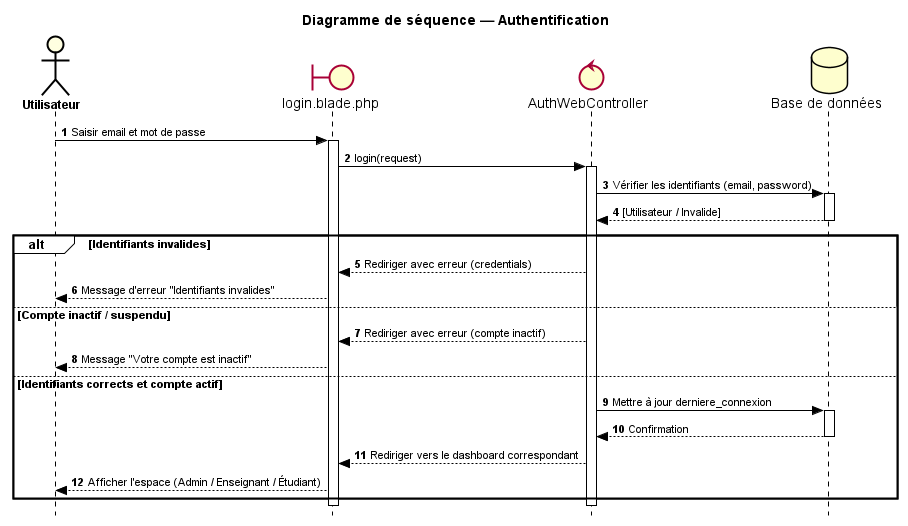
\includegraphics[width=0.8\textwidth]{figures/AUTHENTIFCATION.png}
    \caption{Diagramme de séquence : Authentification}
    \label{fig:seq_auth}
\end{figure}

\subsection{Diagramme de séquence : Inscription à un cours}
Ce cas d'utilisation permet à un étudiant de s'inscrire à un cours disponible en utilisant une clé d'inscription fournie par l'enseignant. L'étudiant sélectionne un cours dans le catalogue et clique sur "S'inscrire". Le système affiche un formulaire modal demandant la clé d'inscription. L'étudiant saisit la clé, puis le système vérifie qu'elle correspond à celle enregistrée pour ce cours et que l'étudiant n'est pas déjà inscrit. Si la clé est valide, le système enregistre l'inscription dans la base de données, initialise la progression à 0\% et confirme l'opération. Si la clé est incorrecte, un message d'erreur est affiché.

La figure \ref{fig:seq_inscrip} montre les étapes suivies par un étudiant pour s'inscrire à un cours, incluant la saisie et la vérification de la clé d'inscription, la vérification d'inscription existante et la confirmation de l'opération.

\begin{figure}[H]
    \centering
    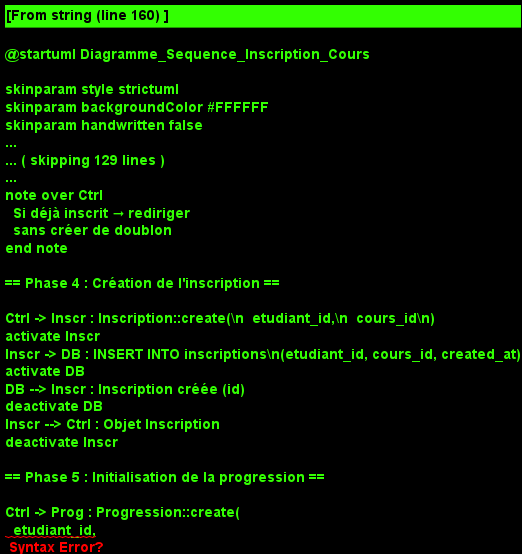
\includegraphics[width=0.8\textwidth]{figures/INSCRIPTION.png}
    \caption{Diagramme de séquence : Inscription à un cours}
    \label{fig:seq_inscrip}
\end{figure}

\subsection{Diagramme de séquence : Participation à un quiz}
Ce cas d'utilisation est le plus complexe et le plus important pour l'étudiant. Il englobe le lancement du quiz, la soumission des réponses et la consultation des résultats. L'étudiant lance un quiz associé à une leçon. Le système récupère les questions du quiz et les présente à l'étudiant. L'étudiant soumet ses réponses, le système les enregistre, met à jour sa progression et calcule le score final. L'étudiant peut ensuite consulter ses résultats pour visualiser son score et sa progression dans le cours.

La figure \ref{fig:seq_quiz} illustre l'intégralité du processus de participation à un quiz, depuis le lancement et la récupération des questions, jusqu'à la soumission des réponses, l'enregistrement, le calcul du score et la consultation des résultats par l'étudiant.

\begin{figure}[H]
    \centering
    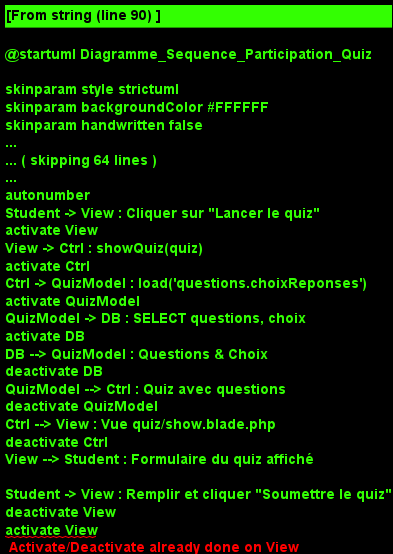
\includegraphics[width=0.9\textwidth]{figures/participerquiz.png}
    \caption{Diagramme de séquence : Participation à un quiz}
    \label{fig:seq_quiz}
\end{figure}

\subsection{Diagramme de séquence : Création d'un cours par l'enseignant}
La gestion des cours est une fonctionnalité centrale pour l'enseignant. Elle lui permet de créer du contenu pédagogique. L'enseignant, après s'être authentifié, accède à son espace de gestion des cours. Il saisit les informations du cours, notamment le titre, la description et les objectifs. Le système valide les données, crée le cours en base de données et confirme l'opération à l'enseignant.

La figure \ref{fig:seq_create_cours} décrit les interactions entre l'enseignant et le système lors de la création d'un nouveau cours, depuis la saisie des informations jusqu'à la confirmation.

\begin{figure}[H]
    \centering
    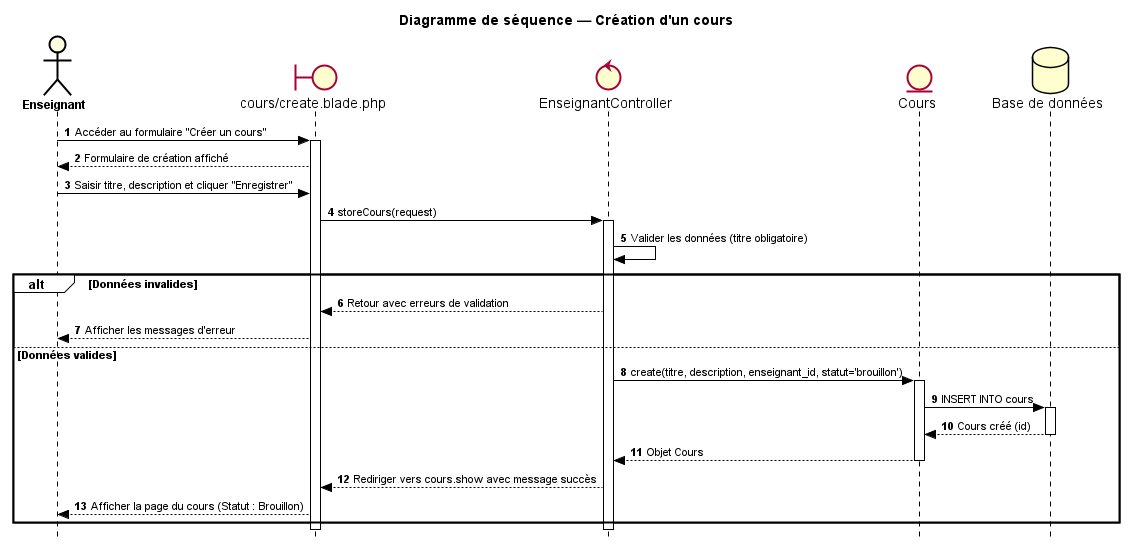
\includegraphics[width=0.8\textwidth]{figures/creation.png}
    \caption{Diagramme de séquence : Création d'un cours par l'enseignant}
    \label{fig:seq_create_cours}
\end{figure}

\subsection{Diagramme de séquence : Modification d'un cours}
L'enseignant peut modifier les informations d'un cours existant. Il sélectionne le cours à modifier, saisit les nouvelles informations et soumet les changements. Le système vérifie l'existence du cours, met à jour les données dans la base et confirme la modification à l'enseignant.

La figure \ref{fig:seq_mod_cours} illustre le processus de modification des informations d'un cours existant par l'enseignant.

\begin{figure}[H]
    \centering
    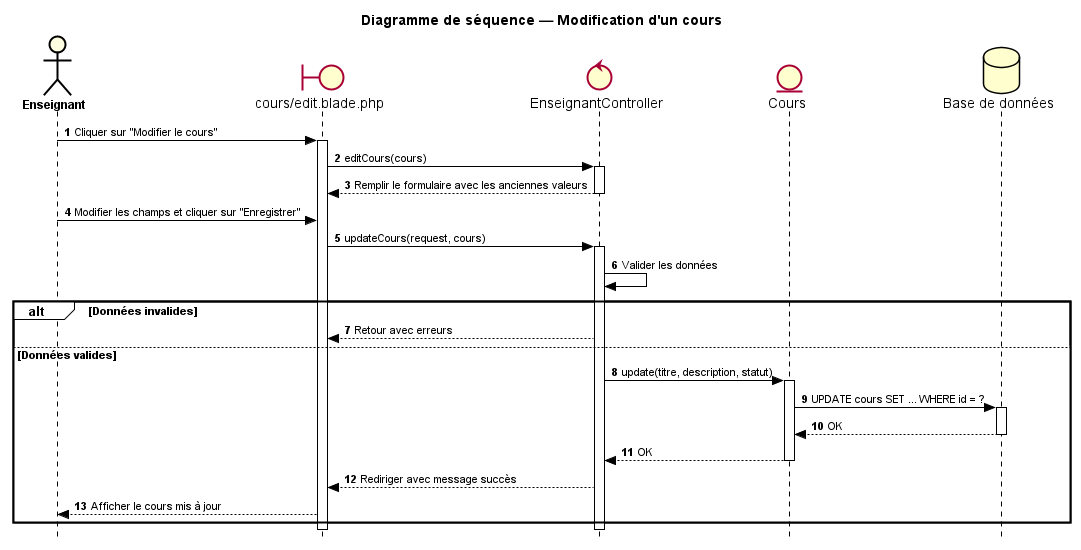
\includegraphics[width=0.8\textwidth]{figures/modification.png}
    \caption{Diagramme de séquence : Modification d'un cours}
    \label{fig:seq_mod_cours}
\end{figure}

\subsection{Diagramme de séquence : Suppression d'un cours}
L'enseignant peut supprimer un cours dont il est l'auteur. Le système vérifie d'abord les dépendances du cours, notamment les leçons, quiz et inscriptions qui lui sont associés. Si des dépendances existent, le système demande une confirmation à l'enseignant pour une suppression en cascade. Après confirmation, le système procède à la suppression de toutes les entités liées et confirme l'opération.

La figure \ref{fig:seq_del_cours} montre la suppression d'un cours avec vérification des dépendances (leçons, quiz, inscriptions) et demande de confirmation avant suppression en cascade.

\begin{figure}[H]
    \centering
    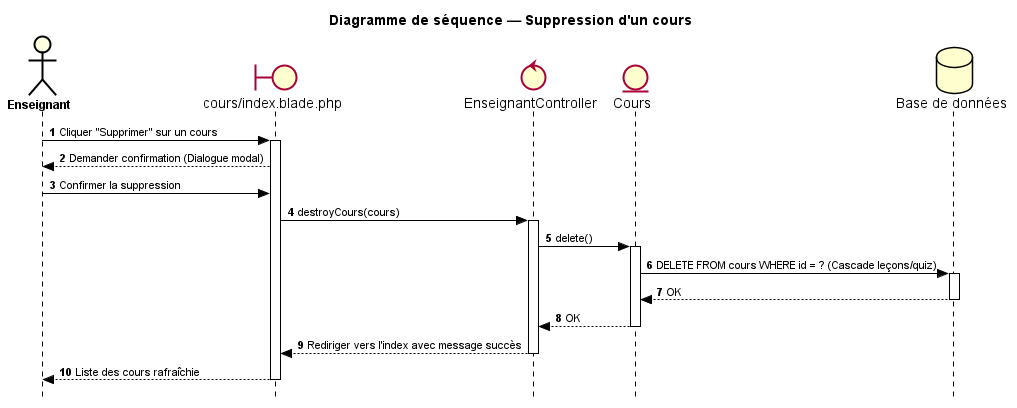
\includegraphics[width=0.8\textwidth]{figures/suppression.png}
    \caption{Diagramme de séquence : Suppression d'un cours}
    \label{fig:seq_del_cours}
\end{figure}

\subsection{Diagramme de séquence : Création d'un quiz avec questions}
Ce cas d'utilisation montre comment un enseignant construit un quiz en ajoutant successivement des questions. L'enseignant crée d'abord le quiz pour une leçon en fournissant le titre. Ensuite, il ajoute les questions une par une avec leur texte, leur type, les options éventuelles pour les QCM et la réponse correcte. Le système persiste chaque élément au fur et à mesure de leur création.

La figure \ref{fig:seq_create_quiz} présente la construction progressive d'un quiz par l'enseignant, incluant l'ajout successif des questions avec leurs paramètres.

\begin{figure}[H]
    \centering
    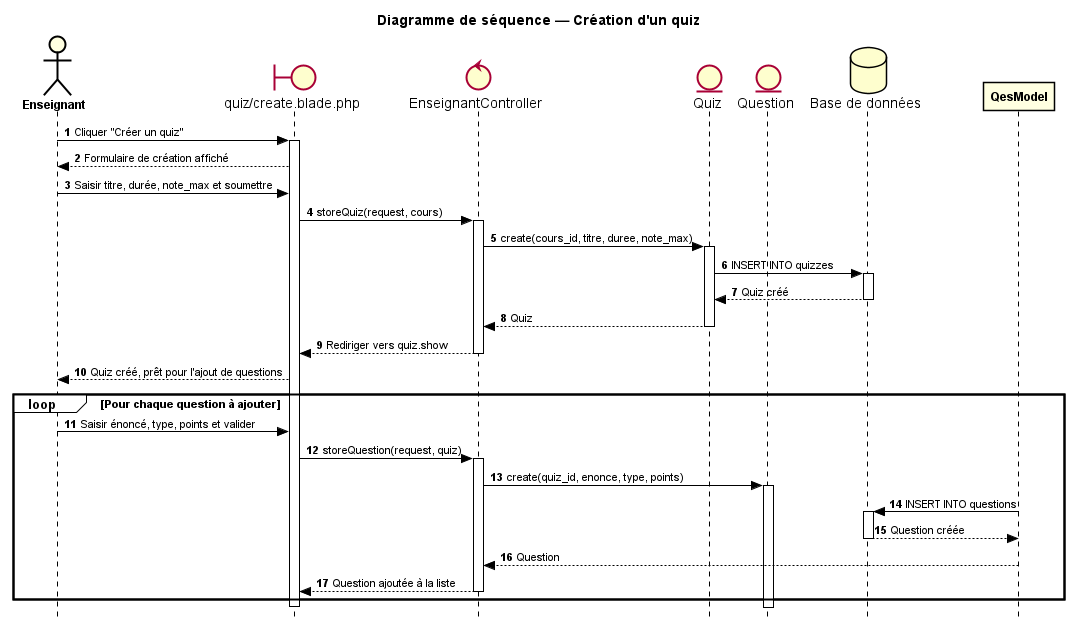
\includegraphics[width=0.8\textwidth]{figures/creationquiz.png}
    \caption{Diagramme de séquence : Création d'un quiz avec questions}
    \label{fig:seq_create_quiz}
\end{figure}

\subsection{Diagramme de séquence : Gestion des utilisateurs par l'administrateur}
L'administrateur a la responsabilité de gérer les comptes utilisateurs et de superviser le système. Il peut effectuer plusieurs opérations, notamment l'activation ou la désactivation d'un compte existant. Pour l'activation ou la désactivation, l'administrateur modifie simplement le statut du compte concerné.

La figure \ref{fig:seq_users} illustre l'activation ou la désactivation d'un compte utilisateur par l'administrateur.

\begin{figure}[H]
    \centering
    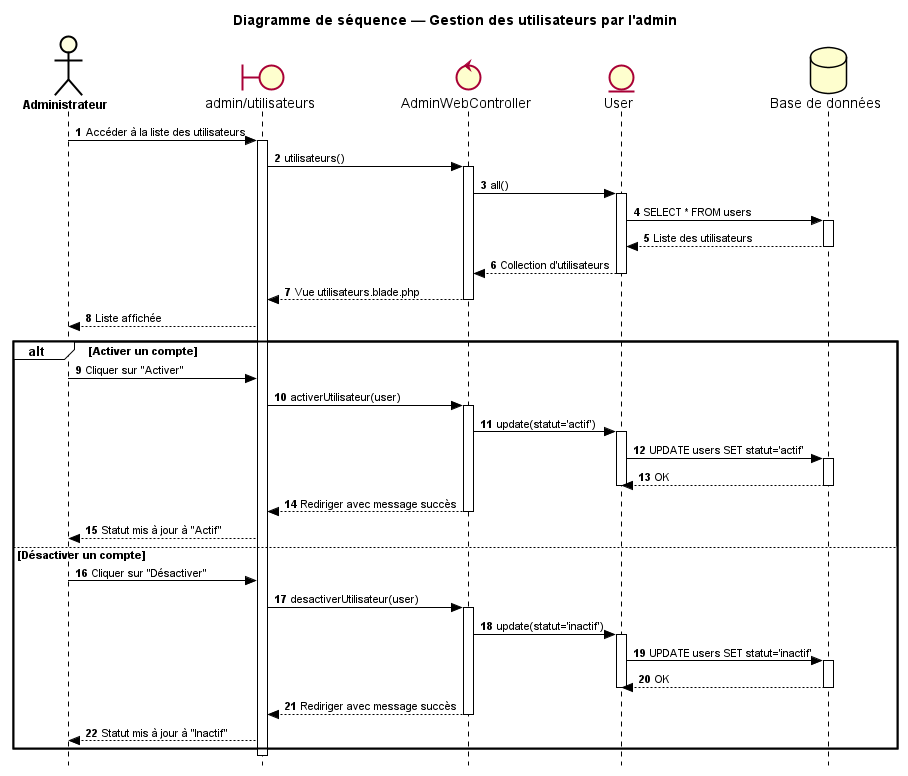
\includegraphics[width=0.9\textwidth]{figures/gestionutilisateur.png}
    \caption{Diagramme de séquence : Gestion des utilisateurs par l'administrateur}
    \label{fig:seq_users}
\end{figure}

\subsection{Diagramme de séquence : Consultation des statistiques globales}
Ce cas permet à l'administrateur d'avoir une vue d'ensemble sur l'activité du système. L'administrateur demande les statistiques globales. Le système agrège les données de la base de données en calculant le nombre d'utilisateurs par rôle, le nombre de cours, le nombre de quiz et le taux de participation. Le système affiche ensuite ces statistiques sous forme de dashboard pour une visualisation claire et synthétique.

La figure \ref{fig:seq_stats} décrit l'agrégation des données par le système (nombre d'utilisateurs, cours, quiz, taux de participation) et leur affichage sous forme de tableau de bord.

\begin{figure}[H]
    \centering
    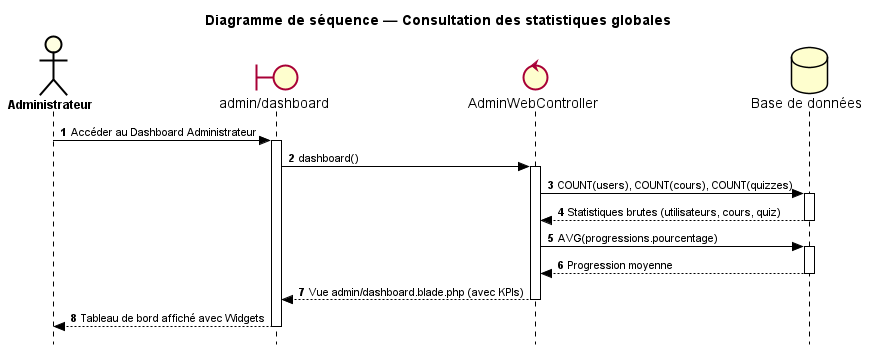
\includegraphics[width=0.9\textwidth]{figures/statistiques.png}
    \caption{Diagramme de séquence : Consultation des statistiques globales}
    \label{fig:seq_stats}
\end{figure}

\subsection{Diagramme de séquence : Correction d'une copie de quiz par l'enseignant}
L'enseignant est notifié des copies en attente de correction. Il sélectionne la copie d'un étudiant spécifique. Le système récupère l'ensemble des réponses (QCM, Vrai/Faux auto-corrigées et Texte libre en attente) et les affiche dans un tableau de bord dédié. L'enseignant attribue manuellement un score et un statut de validation (Correct/Incorrect) aux questions ouvertes, puis soumet sa correction. Le système enregistre les nouvelles notes, recalcule le score total de l'étudiant pour ce quiz, met à jour sa progression globale dans le cours et confirme la sauvegarde à l'enseignant.

La figure \ref{fig:seq_correction} détaille ce processus itératif de récupération des réponses non évaluées, de saisie des scores par l'enseignant et de mise à jour des données de l'étudiant.

\begin{figure}[H]
    \centering
    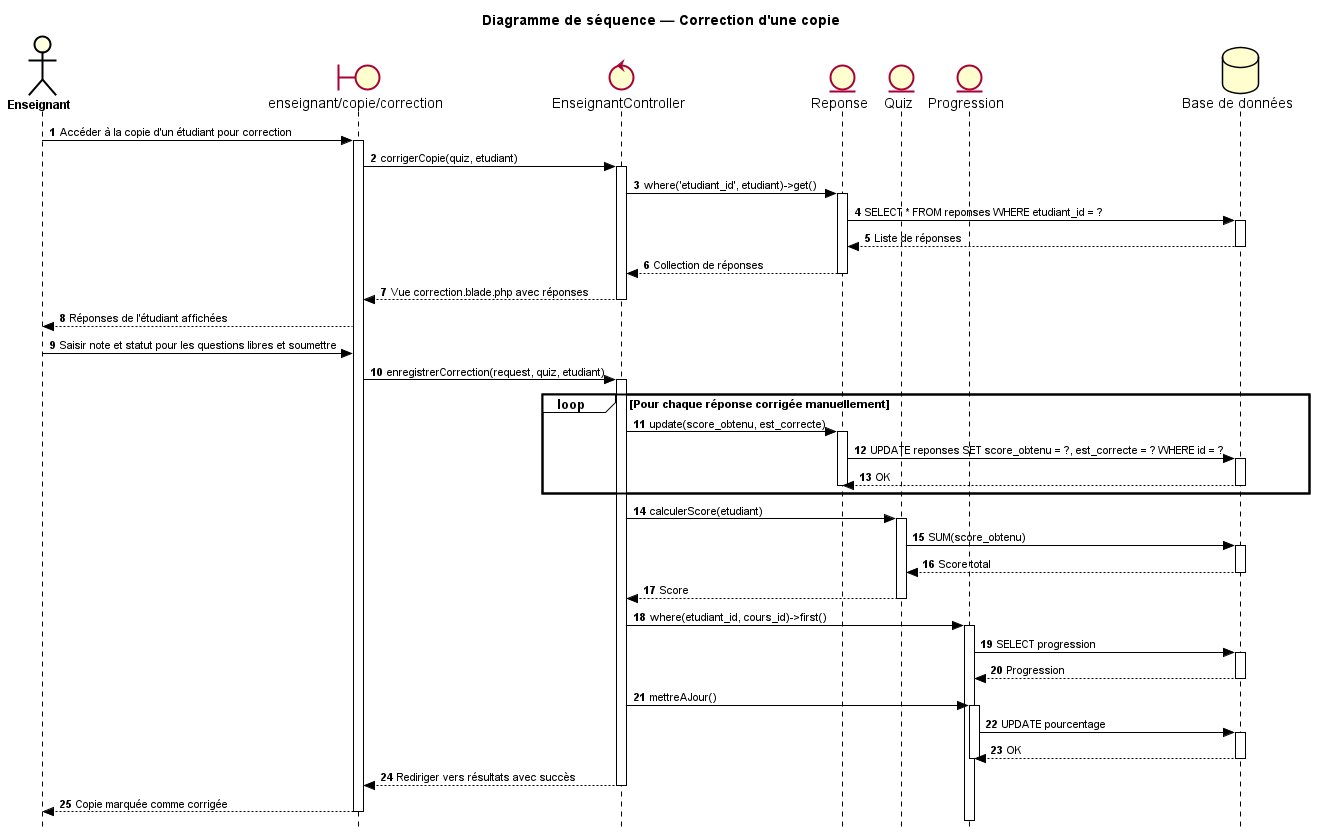
\includegraphics[width=0.9\textwidth]{figures/correction_copie.png}
    \caption{Diagramme de séquence : Correction d'une copie de quiz}
    \label{fig:seq_correction}
\end{figure}

\section{Construction du modèle du domaine}
Le modèle du domaine représente les concepts clés du système et les relations entre eux. Il constitue le cœur de la logique métier et servira de base pour l'implémentation. Cette section présente le diagramme de classes du domaine en précisant les attributs des classes, leurs opérations et les relations entre elles.

\subsection{Diagramme de classes du domaine}
La figure \ref{fig:class_domain} illustre le modèle conceptuel du système avec les entités principales (Utilisateur, Cours, Leçon, Quiz, Question, Réponse, Inscription, Progression), leurs attributs, opérations et relations.

\clearpage
\fancyhead[L]{}
\fancyfoot[C]{}
\renewcommand{\headrulewidth}{0pt}
\renewcommand{\footrulewidth}{0pt}
\begin{sidewaysfigure}
    \centering
    \includegraphics[width=0.85\textheight]{figures/classe.png}
    \caption{Diagramme de classes du domaine}
    \label{fig:class_domain}
    \vspace{2cm}
    \thepage
\end{sidewaysfigure}
\clearpage
\fancyhead[L]{\leftmark}
\fancyfoot[C]{\thepage}
\renewcommand{\headrulewidth}{0.4pt}
\renewcommand{\footrulewidth}{0.4pt}

\subsection{Description des classes}
La classe \textbf{Utilisateur} est une classe abstraite qui regroupe les attributs et méthodes communs à tous les acteurs du système. Elle constitue la racine de l'héritage pour les trois types d'utilisateurs que sont l'Administrateur, l'Enseignant et l'Étudiant. Ses attributs principaux sont l'identifiant unique, le nom, l'email qui sert également d'identifiant de connexion, le mot de passe hashé et le rôle qui détermine les permissions de l'utilisateur dans le système. Les méthodes communes incluent la connexion, la déconnexion et la modification du profil.

La classe \textbf{Administrateur} hérite de Utilisateur et représente les gestionnaires du système. Elle n'ajoute pas d'attributs spécifiques car l'administrateur hérite de tous les attributs de base, mais elle dispose de permissions étendues pour la gestion des comptes et la supervision globale.

La classe \textbf{Enseignant} hérite de Utilisateur et représente les créateurs de contenu pédagogique. Elle ajoute deux attributs spécifiques que sont la spécialité, qui indique le domaine d'expertise de l'enseignant, et la bio, qui permet une présentation personnelle. Les méthodes de cette classe reflètent ses responsabilités dans le système, notamment la création, la modification et la suppression de cours, la création de leçons, la création de quiz, l'ajout de questions, la correction des quiz et la consultation des résultats des étudiants.

La classe \textbf{Étudiant} hérite de Utilisateur et représente les apprenants qui suivent les cours. Elle ajoute l'attribut niveau pour indiquer le niveau d'étude ou la classe de l'étudiant. Ses méthodes lui permettent de consulter les cours, de passer les quiz, de voir sa progression et de consulter l'historique de ses résultats.

La classe \textbf{Cours} représente une unité d'apprentissage principale créée par un enseignant. Ses attributs comprennent un identifiant unique, un titre, une description, la date de création, un statut indiquant si le cours est publié ou archivé, et une clé d'inscription unique générée par l'enseignant pour contrôler l'accès des étudiants. Les méthodes associées permettent de publier ou d'archiver le cours.

La classe \textbf{Leçon} représente une composante d'un cours. Elle possède un identifiant, un titre, un contenu pédagogique qui peut inclure du texte, des vidéos ou d'autres ressources, un type indiquant la nature de la leçon et des points attribués.

La classe \textbf{Quiz} représente une évaluation associée à un cours. Ses attributs sont l'identifiant, le titre, la durée limite éventuelle et la note maximale. Les méthodes permettent de calculer le score d'un étudiant et d'effectuer une correction automatique pour les questions qui le permettent.

La classe \textbf{Question} représente un élément d'un quiz. Elle possède un énoncé, un type qui peut être QCM, vrai/faux ou texte libre, et un nombre de points attribués. 

La classe \textbf{ChoixReponse} représente une option de réponse pour une question de type QCM. Elle possède un contenu textuel et un indicateur booléen précisant si c'est la bonne réponse ou non.

La classe \textbf{Réponse} représente la soumission d'un étudiant à une question. Elle contient le contenu de la réponse soumise, un indicateur de correction pour les réponses automatiques, la date de soumission et le score obtenu. 

La classe \textbf{Inscription} représente la relation formelle entre un étudiant et un cours. Elle contient l'identifiant de l'inscription et la date à laquelle l'étudiant s'est inscrit au cours.

La classe \textbf{Progression} représente l'avancement d'un étudiant dans un cours. Elle contient le pourcentage de progression calculé et la date de dernière mise à jour.

La classe \textbf{LeconVue} est une classe de traçabilité qui enregistre lorsqu'un étudiant a consulté une leçon spécifique d'un cours, permettant de déclencher la mise à jour de la progression.

\subsection{Relations entre les classes}
Un Utilisateur peut être spécialisé en Étudiant, Enseignant ou Administrateur, ce qui est représenté par une relation d'héritage où les classes filles héritent de tous les attributs et méthodes de la classe mère.

Un Enseignant peut créer plusieurs Cours, tandis qu'un Cours est créé par un seul Enseignant. Cette relation bidirectionnelle est essentielle pour assurer la traçabilité du contenu pédagogique.

Un Cours peut contenir plusieurs Leçons, et une Leçon appartient à un seul Cours. La suppression d'un Cours entraîne la suppression de ses Leçons pour maintenir la cohérence des données.

Un Cours peut également contenir plusieurs Quiz, et un Quiz appartient à un seul Cours (non pas à la leçon).

Un Quiz peut contenir plusieurs Questions, et une Question appartient à un seul Quiz. 
Une Question de type QCM peut posséder plusieurs Choix de Réponses (ChoixReponse).

Un Étudiant peut soumettre plusieurs Réponses, et une Réponse est soumise par un seul Étudiant pour une seule Question.

Un Étudiant peut s'inscrire à plusieurs Cours, implémenté par la classe d'association Inscription.

La classe LeconVue trace le fait qu'un Étudiant a visualisé une Leçon particulière d'un Cours.

La Progression est calculée et liée à un Étudiant et à un Cours spécifique (et non directement à l'inscription).

\section{Architecture du futur logiciel}
Pour garantir la maintenabilité, l'évolutivité et la testabilité de notre application, nous adoptons une architecture en couches de type MVC, acronyme de Modèle-Vue-Contrôleur. Cette architecture sépare clairement les responsabilités en trois composants distincts. Le Modèle représente la logique métier et les données de l'application, gérant l'accès à la base de données, les règles de gestion et les validations. La Vue correspond à l'interface utilisateur et présente les données aux utilisateurs tout en capturant leurs actions. Le Contrôleur fait le lien entre le Modèle et la Vue en recevant les requêtes des utilisateurs, en les traitant via les services du Modèle, puis en sélectionnant la Vue appropriée pour afficher la réponse.

Cette architecture présente plusieurs avantages. La séparation des préoccupations permet une meilleure organisation du code et facilite la maintenance. La testabilité est améliorée car chaque couche peut être testée indépendamment. La réutilisabilité des composants métier est accrue, et l'évolutivité du système est facilitée par le faible couplage entre les couches.

Notre implémentation s'appuie sur le framework Laravel, qui propose une architecture MVC enrichie par plusieurs composants supplémentaires assurant la robustesse et la flexibilité du système.

Le système de routage de Laravel constitue le point d'entrée de toutes les requêtes HTTP. Il associe chaque URL à un contrôleur spécifique et applique les middlewares de sécurité et de contrôle d'accès. Dans notre application, les routes sont organisées par groupe selon le rôle de l'utilisateur (administrateur, enseignant, étudiant), ce qui permet une gestion centralisée des permissions d'accès.

Les middlewares sont des composants qui interceptent les requêtes HTTP avant qu'elles n'atteignent les contrôleurs. Ils jouent un rôle essentiel dans notre architecture en assurant l'authentification des utilisateurs et la vérification des rôles. Chaque requête passe d'abord par le middleware d'authentification qui vérifie que l'utilisateur est connecté, puis par le middleware de rôle qui s'assure que l'utilisateur dispose des permissions nécessaires pour accéder à la ressource demandée.

Eloquent est l'ORM (Object-Relational Mapping) intégré de Laravel. Il permet d'interagir avec la base de données MySQL en utilisant des objets PHP au lieu de requêtes SQL brutes. Chaque table de la base de données est représentée par un modèle Eloquent qui encapsule la logique d'accès aux données, les relations entre les entités et les règles de validation. Cette approche orientée objet facilite la maintenance du code et réduit les risques d'erreurs liées à l'écriture manuelle de requêtes SQL.

Blade est le moteur de templates de Laravel utilisé pour générer les vues HTML. Il offre une syntaxe concise et expressive pour afficher les données, gérer les boucles, les conditions et inclure des composants réutilisables. Dans notre application, Blade permet de créer une interface utilisateur cohérente grâce à un système de layouts et de composants partagés entre les différentes pages.

Les policies (politiques) sont des classes qui centralisent la logique d'autorisation pour chaque modèle de l'application. Elles définissent quelles actions un utilisateur peut effectuer sur une ressource donnée. Par exemple, une policy associée au modèle Cours détermine si un utilisateur peut modifier ou supprimer un cours en fonction de son rôle et de sa relation avec le cours concerné. Cette approche garantit que les règles d'accès sont appliquées de manière uniforme dans toute l'application.

Le traitement d'une requête dans notre architecture suit un parcours bien défini. Lorsqu'un utilisateur effectue une action dans le navigateur, une requête HTTP est envoyée au serveur. Le routeur Laravel analyse l'URL et la méthode HTTP pour identifier le contrôleur et la méthode à invoquer. Les middlewares appliquent ensuite les vérifications de sécurité. Si l'utilisateur est autorisé, le contrôleur traite la requête en faisant appel aux modèles Eloquent pour accéder aux données. Les résultats sont ensuite transmis à une vue Blade qui génère la réponse HTML envoyée au navigateur de l'utilisateur.

Ce flux de traitement assure une séparation claire entre la gestion des requêtes, la logique métier, l'accès aux données et la présentation, conformément aux principes de l'architecture MVC.

\section{Schémas physiques des données}
À partir du diagramme de classes du domaine, nous dérivons le schéma physique de la base de données. Ce schéma décrit la structure concrète des tables avec leurs colonnes, types, contraintes et relations. Nous utilisons MySQL comme système de gestion de base de données.

\subsection{Table Utilisateur}
La table \texttt{users} stocke les informations d'authentification communes, tandis que \texttt{enseignants} et \texttt{etudiants} gèrent les informations spécifiques aux rôles respectifs.

\begin{lstlisting}[language=SQL]
CREATE TABLE users (
    id BIGINT UNSIGNED PRIMARY KEY AUTO_INCREMENT,
    nom VARCHAR(255) NOT NULL,
    prenom VARCHAR(255) NOT NULL,
    email VARCHAR(255) UNIQUE NOT NULL,
    email_verified_at TIMESTAMP NULL,
    mot_de_passe VARCHAR(255) NOT NULL,
    role ENUM('etudiant', 'enseignant', 'administrateur') NOT NULL,
    actif BOOLEAN DEFAULT false,
    remember_token VARCHAR(100) NULL,
    created_at TIMESTAMP NULL,
    updated_at TIMESTAMP NULL
);

CREATE TABLE enseignants (
    id BIGINT UNSIGNED PRIMARY KEY AUTO_INCREMENT,
    user_id BIGINT UNSIGNED NOT NULL,
    specialite VARCHAR(255) NOT NULL,
    bio TEXT NULL,
    created_at TIMESTAMP NULL,
    updated_at TIMESTAMP NULL,
    FOREIGN KEY (user_id) REFERENCES users(id) ON DELETE CASCADE
);

CREATE TABLE etudiants (
    id BIGINT UNSIGNED PRIMARY KEY AUTO_INCREMENT,
    user_id BIGINT UNSIGNED NOT NULL,
    niveau VARCHAR(255) NOT NULL,
    created_at TIMESTAMP NULL,
    updated_at TIMESTAMP NULL,
    FOREIGN KEY (user_id) REFERENCES users(id) ON DELETE CASCADE
);
\end{lstlisting}

\subsection{Table Cours}
La table Cours contient les informations sur les cours créés par les enseignants. Elle comprend un identifiant unique, le titre du cours, sa description, une référence à l'enseignant qui a créé le cours, un statut et une clé d'inscription unique utilisée par les étudiants pour s'inscrire. La clé étrangère vers l'enseignant assure l'intégrité référentielle et la suppression en cascade garantit la cohérence des données.

\begin{lstlisting}[language=SQL]
CREATE TABLE cours (
    id BIGINT UNSIGNED PRIMARY KEY AUTO_INCREMENT,
    enseignant_id BIGINT UNSIGNED NOT NULL,
    titre VARCHAR(255) NOT NULL,
    description TEXT NULL,
    statut ENUM('brouillon', 'publie', 'archive') DEFAULT 'brouillon',
    cle_inscription VARCHAR(10) NULL UNIQUE,
    created_at TIMESTAMP NULL,
    updated_at TIMESTAMP NULL,
    FOREIGN KEY (enseignant_id) REFERENCES enseignants(id) ON DELETE CASCADE
);
\end{lstlisting}

\subsection{Table Leçon}
\begin{lstlisting}[language=SQL]
CREATE TABLE lecons (
    id BIGINT UNSIGNED PRIMARY KEY AUTO_INCREMENT,
    cours_id BIGINT UNSIGNED NOT NULL,
    titre VARCHAR(255) NOT NULL,
    contenu TEXT NOT NULL,
    type ENUM('video', 'texte', 'pdf', 'presentation') NOT NULL,
    ordre INT NOT NULL,
    created_at TIMESTAMP NULL,
    updated_at TIMESTAMP NULL,
    FOREIGN KEY (cours_id) REFERENCES cours(id) ON DELETE CASCADE
);
\end{lstlisting}

\subsection{Table Quiz}
La table \texttt{quizzes} contient les évaluations associées aux cours. La clé étrangère vers le cours (\texttt{cours\_id}) assure la liaison directe.

\begin{lstlisting}[language=SQL]
CREATE TABLE quizzes (
    id BIGINT UNSIGNED PRIMARY KEY AUTO_INCREMENT,
    cours_id BIGINT UNSIGNED NOT NULL,
    titre VARCHAR(255) NOT NULL,
    duree INT NOT NULL COMMENT 'Durée en minutes',
    note_max INT NOT NULL,
    created_at TIMESTAMP NULL,
    updated_at TIMESTAMP NULL,
    FOREIGN KEY (cours_id) REFERENCES cours(id) ON DELETE CASCADE
);
\end{lstlisting}

\subsection{Table Question}
\begin{lstlisting}[language=SQL]
CREATE TABLE questions (
    id BIGINT UNSIGNED PRIMARY KEY AUTO_INCREMENT,
    quiz_id BIGINT UNSIGNED NOT NULL,
    enonce TEXT NOT NULL,
    type ENUM('qcm', 'vrai_faux', 'texte_libre') NOT NULL,
    points INT NOT NULL,
    reponse_attendue TEXT NULL,
    created_at TIMESTAMP NULL,
    updated_at TIMESTAMP NULL,
    FOREIGN KEY (quiz_id) REFERENCES quizzes(id) ON DELETE CASCADE
);

CREATE TABLE choix_reponses (
    id BIGINT UNSIGNED PRIMARY KEY AUTO_INCREMENT,
    question_id BIGINT UNSIGNED NOT NULL,
    contenu TEXT NOT NULL,
    est_correcte BOOLEAN NOT NULL,
    created_at TIMESTAMP NULL,
    updated_at TIMESTAMP NULL,
    FOREIGN KEY (question_id) REFERENCES questions(id) ON DELETE CASCADE
);
\end{lstlisting}

\subsection{Table Réponse}
\begin{lstlisting}[language=SQL]
CREATE TABLE reponses (
    id BIGINT UNSIGNED PRIMARY KEY AUTO_INCREMENT,
    etudiant_id BIGINT UNSIGNED NOT NULL,
    question_id BIGINT UNSIGNED NOT NULL,
    contenu TEXT NOT NULL,
    est_correcte BOOLEAN NOT NULL,
    date_reponse TIMESTAMP DEFAULT CURRENT_TIMESTAMP,
    score_obtenu INT NOT NULL,
    created_at TIMESTAMP NULL,
    updated_at TIMESTAMP NULL,
    FOREIGN KEY (etudiant_id) REFERENCES etudiants(id) ON DELETE CASCADE,
    FOREIGN KEY (question_id) REFERENCES questions(id) ON DELETE CASCADE,
    UNIQUE KEY unique_reponse (etudiant_id, question_id)
);
\end{lstlisting}

\subsection{Table Inscription}
La table \texttt{inscriptions} stocke le fait que l'étudiant participe au cours.

\begin{lstlisting}[language=SQL]
CREATE TABLE inscriptions (
    id BIGINT UNSIGNED PRIMARY KEY AUTO_INCREMENT,
    etudiant_id BIGINT UNSIGNED NOT NULL,
    cours_id BIGINT UNSIGNED NOT NULL,
    date_inscription TIMESTAMP DEFAULT CURRENT_TIMESTAMP,
    created_at TIMESTAMP NULL,
    updated_at TIMESTAMP NULL,
    FOREIGN KEY (etudiant_id) REFERENCES etudiants(id) ON DELETE CASCADE,
    FOREIGN KEY (cours_id) REFERENCES cours(id) ON DELETE CASCADE
);
\end{lstlisting}

\subsection{Table Progression}
Les tables \texttt{progressions} et \texttt{lecons\_vues} suivent l'avancement. \texttt{progressions} stocke le pourcentage, et \texttt{lecons\_vues} marque de manière granulaire chaque leçon terminée.

\begin{lstlisting}[language=SQL]
CREATE TABLE progressions (
    id BIGINT UNSIGNED PRIMARY KEY AUTO_INCREMENT,
    etudiant_id BIGINT UNSIGNED NOT NULL,
    cours_id BIGINT UNSIGNED NOT NULL,
    pourcentage INT NOT NULL,
    date_maj TIMESTAMP DEFAULT CURRENT_TIMESTAMP,
    created_at TIMESTAMP NULL,
    updated_at TIMESTAMP NULL,
    FOREIGN KEY (etudiant_id) REFERENCES etudiants(id) ON DELETE CASCADE,
    FOREIGN KEY (cours_id) REFERENCES cours(id) ON DELETE CASCADE
);

CREATE TABLE lecons_vues (
    id BIGINT UNSIGNED PRIMARY KEY AUTO_INCREMENT,
    etudiant_id BIGINT UNSIGNED NOT NULL,
    cours_id BIGINT UNSIGNED NOT NULL,
    lecon_id BIGINT UNSIGNED NOT NULL,
    created_at TIMESTAMP NULL,
    updated_at TIMESTAMP NULL,
    FOREIGN KEY (etudiant_id) REFERENCES etudiants(id) ON DELETE CASCADE,
    FOREIGN KEY (cours_id) REFERENCES cours(id) ON DELETE CASCADE,
    FOREIGN KEY (lecon_id) REFERENCES lecons(id) ON DELETE CASCADE
);
\end{lstlisting}

\section{Conclusion}
Ce chapitre d'analyse et de conception a permis de poser des bases techniques rigoureuses pour notre plateforme LMS. Grâce à l'élaboration des diagrammes de séquence UML, du diagramme de classes du domaine, de l'adoption de l'architecture MVC et de la dérivation du schéma physique de la base de données, nous disposons d'une conception technique claire et cohérente. L'ensemble de ces modélisations fonctionnelles et structurelles constitue le socle indispensable pour entamer sereinement la phase d'implémentation et de développement, qui sera détaillée dans le chapitre suivant.


% Chapitre 4
\chapter{Implémentation}

\section{Introduction}
Ce chapitre présente les aspects techniques de la réalisation du système web léger de gestion de l'apprentissage (LMS). Nous détaillerons l'environnement de développement choisi, les technologies utilisées, ainsi que la mise en œuvre concrète des principaux cas d'utilisation. L'objectif est de montrer comment les spécifications définies dans les chapitres précédents ont été traduites en une application fonctionnelle répondant aux besoins exprimés dans le cahier des charges. Ce chapitre mettra également en lumière les choix techniques effectués et leur justification, ainsi que les captures d'écran illustrant les différentes interfaces développées.

\section{Environnement de réalisation}
La phase d'implémentation du système web léger de gestion de l'apprentissage (LMS) a nécessité la mise en place d'un environnement de développement adapté aux contraintes techniques définies dans le cahier des charges. Le choix des technologies a été guidé par la nécessité d'obtenir une solution robuste, maintenable et conforme aux standards actuels du développement web.

Côté backend, nous avons opté pour le langage PHP dans sa version 8.2, associé au framework Laravel 11. Ce choix s'explique par la maturité du langage PHP, sa large communauté et sa parfaite adéquation avec les contraintes techniques imposées. Laravel, quant à lui, a été retenu pour son architecture MVC (Modèle-Vue-Contrôleur) qui facilite la séparation des préoccupations, son ORM Eloquent qui simplifie les interactions avec la base de données, et son système d'authentification intégré qui garantit une gestion sécurisée des utilisateurs. Ce framework offre également un routage puissant, un système de migration de base de données, et une gestion efficace des dépendances via Composer.

Pour la base de données, nous avons utilisé MySQL dans sa version 8.0, conformément aux spécifications du cahier des charges. Ce système de gestion de base de données relationnelle a été choisi pour sa fiabilité, ses performances, et sa compatibilité avec Laravel. La modélisation des données repose sur une structure comprenant les tables principales suivantes : users pour la gestion des comptes (administrateur, enseignant, étudiant), courses pour le stockage des informations relatives aux cours, leçons pour les leçons associées à chaque cours, quizzes et questions pour les évaluations, ainsi que inscriptions et soumissions pour le suivi des inscriptions et des résultats. Ces tables sont liées par des relations définies à l'aide de clés étrangères, garantissant ainsi l'intégrité référentielle des données.

En ce qui concerne le frontend, nous avons adopté une approche basée sur HTML5, CSS3 et JavaScript standard. Pour la mise en page et le design des interfaces, nous avons utilisé le framework CSS Bootstrap 5, qui nous a permis de développer une interface utilisateur responsive, adaptée à tous les types d'écrans (ordinateurs, tablettes, smartphones), tout en assurant une expérience utilisateur fluide et intuitive. L'interactivité des pages a été implémentée en JavaScript pur, sans recours à des bibliothèques ou frameworks supplémentaires, ce qui garantit une légèreté optimale et une compatibilité avec tous les navigateurs modernes. Le moteur de templates Blade de Laravel a été utilisé pour la génération dynamique des vues, offrant une syntaxe élégante et une intégration native avec le framework.

Pour les outils de développement, nous avons utilisé Visual Studio Code comme environnement de développement intégré, avec des extensions dédiées à PHP et Laravel. La gestion de version a été assurée par Git, permettant un suivi rigoureux des modifications. Composer a servi à la gestion des dépendances PHP, tandis que NPM a été utilisé pour les paquets frontend (Bootstrap essentiellement). L'administration de la base de données a été facilitée par l'utilisation de phpMyAdmin, qui offre une interface graphique intuitive pour la gestion des tables et des données.
% Outils de développement

\section{Outils de développement}

phpMyAdmin est une interface web intuitive qui permet d'administrer facilement la base de données MySQL. Cet outil offre une interface graphique complète pour exécuter des requêtes SQL, créer et modifier des tables, gérer les index et les clés étrangères, et effectuer des opérations de maintenance telles que l'exportation et l'importation de données. Dans le cadre de notre projet, phpMyAdmin a été utilisé quotidiennement pour vérifier l'intégrité des données, tester les requêtes complexes et visualiser les relations entre les tables. Sa facilité d'utilisation et son accessibilité via un simple navigateur en font un outil incontournable pour tout projet basé sur MySQL.
\begin{figure}[H]
    \centering
    \includegraphics[width=0.85\textwidth]{figures/phpmyadmin.png}
    \caption{Logo phpMyAdmin}
\end{figure}

Laravel est le framework PHP moderne utilisé pour développer le LMS. Il offre une architecture MVC complète, un ORM Eloquent performant pour les interactions avec la base de données, un système de migration de données qui facilite le versioning du schéma de base de données, un routage puissant et flexible, et des mécanismes de sécurité intégrés tels que la protection CSRF, le hachage des mots de passe et la prévention des injections SQL. Laravel dispose également d'un système de gestion des dépendances via Composer, d'un moteur de templates Blade, et d'une communauté active qui fournit de nombreuses extensions et packages. La documentation officielle, complète et bien structurée, a été une ressource précieuse tout au long du développement.
\begin{figure}[H]
    \centering
    \includegraphics[width=0.85\textwidth]{figures/laravel.png}
    \caption{logo laravel}
\end{figure}
Visual Studio Code (VS Code) est l’environnement de développement intégré employé pour coder le projet : il propose l’autocomplétion, le debugging, l’intégration Git et des extensions dédiées à PHP et Laravel.
\begin{figure}[H]
    \centering
    \includegraphics[width=0.85\textwidth]{figures/vscode.png}
    \caption{Logo Visual Studio Code}
\end{figure}

Bootstrap 5 est le framework CSS utilisé pour le design et la mise en page des interfaces utilisateur. Il fournit une grille responsive flexible, des composants prêts à l'emploi (boutons, formulaires, cartes, modals, navigation) et un système de thèmes personnalisable. L'utilisation de Bootstrap nous a permis de développer rapidement des interfaces cohérentes et professionnelles, adaptées à tous les types d'écrans grâce au design responsive. La version 5 apporte notamment l'abandon de jQuery en faveur du JavaScript natif, ce qui allège le poids des pages et améliore les performances.

Git est le système de gestion de versions utilisé pour suivre l'historique des modifications du code source. Il permet de travailler de manière collaborative, de créer des branches pour les nouvelles fonctionnalités, et de revenir facilement à une version antérieure en cas de problème. L'utilisation de Git a été essentielle pour maintenir la cohérence du code tout au long du développement et pour documenter l'évolution du projet à travers les messages de commit.

Composer est le gestionnaire de dépendances PHP utilisé pour installer et maintenir les packages Laravel et ses extensions. Il gère automatiquement les versions et les conflits de dépendances. NPM (Node Package Manager) a été utilisé pour gérer les paquets frontend, notamment Bootstrap et les outils de compilation Vite. L'utilisation combinée de ces deux gestionnaires assure une gestion propre et reproductible de l'ensemble des dépendances du projet.

L'architecture technique globale repose sur un modèle client-serveur classique : le navigateur web (client) envoie des requêtes HTTP au serveur Laravel, qui traite ces requêtes via ses contrôleurs, interagit avec la base de données MySQL via l'ORM Eloquent, et retourne des vues générées dynamiquement par Blade. Cette architecture MVC assure une séparation claire entre la logique métier, la gestion des données et la présentation, facilitant ainsi la maintenance et l'évolution future du système. Enfin, la sécurité a été renforcée par l'utilisation de middlewares pour le contrôle d'accès, le hachage des mots de passe avec la fonction native de Laravel, et la protection contre les attaques courantes telles que les injections SQL et les failles CSRF.

\section{Réalisation technique des cas d'utilisation}
Nous présentons dans cette section la réalisation technique des cas d'utilisation majeurs identifiés dans le chapitre de capture des besoins. Pour chaque cas d'utilisation, nous fournissons une description technique détaillée incluant des captures d'écran, des extraits de code et des composants techniques spécifiques.

\subsection{Cas d'utilisation : S'authentifier}
\textbf{Description :} L'utilisateur (Administrateur, Enseignant ou Étudiant) se connecte au système via ses identifiants. Ce cas d'utilisation permet également l'inscription des nouveaux étudiants.

La figure \ref{fig:ui_login} illustre la page de connexion permettant à l'utilisateur de saisir son email et son mot de passe pour accéder au système.

\begin{figure}[H]
    \centering
    \includegraphics[width=0.8\textwidth]{figures/auth.png}
    \caption{Capture d'écran : Interface d'authentification}
    \label{fig:ui_login}
\end{figure}

\textbf{Extrait de code :} Le contrôleur d'authentification gère la tentative de connexion en utilisant le système Auth de Laravel.

\begin{lstlisting}[language=PHP]
// app/Http/Controllers/AuthController.php
public function login(Request $request)
{
    $credentials = $request->validate([
        'email' => 'required|email',
        'password' => 'required',
    ]);

    if (Auth::attempt($credentials)) {
        $request->session()->regenerate();
        return redirect()->intended('dashboard');
    }

    return back()->withErrors([
        'email' => 'Les identifiants fournis ne correspondent pas.',
    ]);
}
\end{lstlisting}
\textbf{Bibliothèques utilisées :} Laravel Auth, Laravel Sanctum pour la gestion des tokens d'authentification.

\subsection{Cas d'utilisation : Gérer les cours}

La figure \ref{fig:ui_liste_cours} illustre l'interface d'affichage de la liste des cours disponibles.

\begin{figure}[H]
    \centering
    \includegraphics[width=1.1\textwidth]{figures/gerer.png}
    \caption{Capture d'écran : Gestion des cours (liste des cours)}
    \label{fig:ui_liste_cours}
\end{figure}

\begin{lstlisting}[language=PHP]
// app/Http/Controllers/CourseController.php
public function store(Request $request)
{
    $validated = $request->validate([
        'title' => 'required|string|max:255',
        'description' => 'required|string',
        'status' => 'required|in:draft,published',
    ]);

    $course = Course::create([
        'title' => $validated['title'],
        'description' => $validated['description'],
        'status' => $validated['status'],
        'teacher_id' => Auth::id(),
    ]);

    return redirect()->route('courses.index')
                     ->with('success', 'Cours créé avec succès.');
}
\end{lstlisting}

La figure \ref{fig:ui_form_cours} illustre le formulaire de création ou de modification d'un cours.

\begin{figure}[H]
    \centering
    \includegraphics[width=1\textwidth]{figures/creationcourscapture.png}
    \caption{Capture d'écran : Gestion des cours (création/modification)}
    \label{fig:ui_form_cours}
\end{figure}

\subsection{Cas d'utilisation : Créer et configurer un quiz}

\textbf{Extrait de code :} Le modèle Quiz établit les relations nécessaires avec les cours et les questions. Ce cas d'utilisation porte sur la création et la configuration initiale d'un quiz, et non sur un processus générique de gestion/édition/suppression de quiz.

\begin{lstlisting}[language=PHP]
// app/Models/Quiz.php
class Quiz extends Model
{
    use HasFactory;

    protected $fillable = ['title', 'duration', 'max_score', 'course_id'];

    public function course()
    {
        return $this->belongsTo(Course::class);
    }

    public function questions()
    {
        return $this->hasMany(Question::class);
    }

    public function results()
    {
        return $this->hasMany(Result::class);
    }
}
\end{lstlisting}
\textbf{Bibliothèques utilisées :} Laravel Eloquent ORM pour la gestion des relations et des requêtes.

\subsection{Cas d'utilisation : Participer à un quiz}

La figure \ref{fig:ui_participation_quiz} présente l'interface interactive permettant à l'étudiant de participer à un quiz. Cette vue affiche clairement l'énoncé de la question en cours ainsi que les différentes options de réponse proposées. L'apprenant peut sélectionner la réponse de son choix avec une navigation fluide tout au long du test.

\begin{figure}[H]
    \centering
    \includegraphics[width=1\textwidth]{figures/participer.png}
    \caption{Capture d'écran : Participation à un quiz}
    \label{fig:ui_participation_quiz}
\end{figure}

Une fois l'ensemble des questions traitées, l'étudiant valide son test. La figure \ref{fig:ui_soumission_quiz} illustre l'écran généré immédiatement après la soumission. Le système calcule automatiquement la note finale en base de données et affiche un résumé instantané des performances de l'étudiant, incluant le score obtenu, ce qui favorise une auto-évaluation rapide et efficace.

\begin{figure}[H]
    \centering
    \includegraphics[width=1\textwidth]{figures/soumission_resultat.png}
    \caption{Capture d'écran : Soumission des réponses et résultats}
    \label{fig:ui_soumission_quiz}
\end{figure}

\textbf{Extrait de code :} Le contrôleur de quiz traite la soumission et calcule automatiquement le score.

\begin{lstlisting}[language=PHP]
// app/Http/Controllers/QuizController.php
public function submit(Request $request, Quiz $quiz)
{
    $answers = $request->input('answers');
    $totalScore = 0;

    foreach ($quiz->questions as $question) {
        $userAnswer = $answers[$question->id] ?? null;
        if ($userAnswer == $question->correct_answer) {
            $totalScore += $question->points;
        }
    }

    $result = Result::create([
        'user_id' => Auth::id(),
        'quiz_id' => $quiz->id,
        'score' => $totalScore,
        'submitted_at' => now(),
    ]);

    return redirect()->route('quiz.results', $quiz)->with('score', $totalScore);
}
\end{lstlisting}

\subsection{Cas d'utilisation : Consulter le tableau de bord}

La figure \ref{fig:ui_dashboard} présente le tableau de bord avec les statistiques globales de la plateforme (nombre d'étudiants, cours, quiz, taux de réussite moyen, etc.).

\begin{figure}[H]
    \centering
    \includegraphics[width=1\textwidth]{figures/tableau.png}
    \caption{Capture d'écran : Tableau de bord administrateur}
    \label{fig:ui_dashboard}
\end{figure}

\textbf{Extrait de code :} Le contrôleur du tableau de bord agrège les données nécessaires via des requêtes Eloquent.

\begin{lstlisting}[language=PHP]
// app/Http/Controllers/DashboardController.php
public function index()
{
    $stats = [
        'total_students' => User::where('role', 'student')->count(),
        'total_courses' => Course::count(),
        'total_quizzes' => Quiz::count(),
        'total_results' => Result::count(),
        'avg_success_rate' => Result::avg('score') ?? 0,
    ];

    $coursesSuccess = Course::with('quizzes.results')
        ->get()
        ->map(function ($course) {
            return [
                'title' => $course->title,
                'avg_score' => $course->quizzes->flatMap->results->avg('score') ?? 0,
            ];
        });

    return view('dashboard.index', compact('stats', 'coursesSuccess'));
}
\end{lstlisting}


La figure \ref{fig:catalogue_cours} présente l'interface d'accueil pour les étudiants et les visiteurs. Elle affiche sous forme de cartes (cards) l'ensemble des cours disponibles sur la plateforme. Chaque carte résume les informations essentielles : le titre du cours, une brève description, le nom de l'enseignant et un bouton permettant d'accéder aux détails ou de s'y inscrire.

\begin{figure}[H]
    \centering
    \includegraphics[width=0.9\textwidth]{figures/catalogue_cours.png}
    \caption{Capture d'écran : Catalogue des cours (Vue Étudiant)}
    \label{fig:catalogue_cours}
\end{figure}

Une fois inscrit, l'étudiant accède à l'espace détaillé du cours, illustré par la figure \ref{fig:details_cours}. Cette interface liste de manière séquentielle toutes les leçons et les quiz rattachés au cours. Elle intègre également une barre de progression dynamique qui se met à jour automatiquement en fonction des leçons validées et des quiz réussis, offrant ainsi un suivi visuel de l'apprentissage.

\begin{figure}[H]
    \centering
    \includegraphics[width=0.9\textwidth]{figures/details_cours.png}
    \caption{Capture d'écran : Détails d'un cours et progression}
    \label{fig:details_cours}
\end{figure}

La figure \ref{fig:profil_utilisateur} montre l'interface de gestion du profil, accessible à tous les utilisateurs (Administrateurs, Enseignants et Étudiants). Elle permet à l'utilisateur de personnaliser ses informations (biographie, spécialité) et de mettre à jour son mot de passe de manière sécurisée. Cette page garantit l'autonomie des utilisateurs sur leurs données personnelles.

\begin{figure}[H]
    \centering
    \includegraphics[width=0.85\textwidth]{figures/profil_utilisateur.png}
    \caption{Capture d'écran : Mise à jour du profil utilisateur}
    \label{fig:profil_utilisateur}
\end{figure}

L'interface d'ajout de leçon, présentée dans la figure \ref{fig:creation_lecon}, est un outil central pour les enseignants. Elle intègre un formulaire riche permettant de définir le titre de la leçon, son ordre dans le cours, et surtout d'insérer le contenu pédagogique (textes, liens, médias) grâce à un éditeur de texte intégré.

\begin{figure}[H]
    \centering
    \includegraphics[width=0.9\textwidth]{figures/creation_lecon.png}
    \caption{Capture d'écran : Ajout d'une leçon par un enseignant}
    \label{fig:creation_lecon}
\end{figure}

La figure \ref{fig:gestion_quiz} illustre l'interface dédiée à la conception des évaluations par l'enseignant. Cette interface complexe mais intuitive permet de configurer les paramètres du quiz (durée, note de passage) et d'y ajouter dynamiquement différents types de questions (Choix multiples, Vrai/Faux) avec leurs réponses respectives.

\begin{figure}[H]
    \centering
    \includegraphics[width=0.9\textwidth]{figures/gestion_quiz.png}
    \caption{Capture d'écran : Configuration des quiz et ajout de questions}
    \label{fig:gestion_quiz}
\end{figure}

\section{Conclusion}
Ce chapitre a présenté l'implémentation technique du système LMS en suivant une approche méthodique et structurée. Nous avons détaillé l'environnement de réalisation avec les technologies choisies : PHP 8.2, Laravel 11, MySQL 8.0, Bootstrap 5 et JavaScript standard. L'architecture MVC a permis une séparation claire des préoccupations, facilitant ainsi la maintenance et l'évolution future du système.

La mise en œuvre des cas d'utilisation a couvert les fonctionnalités essentielles du système :
\begin{itemize}
    \item L'authentification avec gestion des rôles (Administrateur, Enseignant, Étudiant)
    \item La gestion des cours (création, édition, suppression)
    \item La gestion des quiz et des questions d'évaluation
    \item Le tableau de bord administrateur avec statistiques
    \item Le suivi de progression des étudiants
\end{itemize}

Les captures d'écran présentées illustrent les interfaces développées et démontrent la conformité de l'implémentation avec les besoins fonctionnels définis dans le cahier des charges.

L'ensemble de ces travaux constitue une base solide pour la mise en production du système, avec des perspectives d'amélioration telles que l'ajout de fonctionnalités collaboratives, l'intégration d'un système de notification, ou encore le développement d'une application mobile complémentaire.

% Conclusion générale
\clearpage
\addcontentsline{toc}{chapter}{Conclusion générale}
\chapter*{Conclusion générale}
\markboth{Conclusion générale}{Conclusion générale}

Au terme de ce projet de fin d'études, réalisé au sein du groupe MTD Group, nous pouvons affirmer que les objectifs fixés initialement ont été atteints. Notre travail a abouti à la conception et au développement d'un système web léger de gestion de l'apprentissage.

\subsection*{Rappel de l'objet du projet}
Le projet visait à remédier aux difficultés rencontrées dans la gestion des formations, notamment la dispersion des ressources pédagogiques, la charge administrative liée à la correction manuelle des évaluations et l'absence d'outils de suivi de la progression des apprenants. Pour répondre à ces problématiques, nous avons conçu une plateforme centralisée permettant à l'administrateur de superviser l'ensemble du système, aux enseignants de créer et gérer des cours, des leçons et des quiz, et aux étudiants de consulter les ressources pédagogiques, de passer des évaluations et de suivre leur progression personnelle.

\subsection*{Synthèse des travaux réalisés}
La réalisation de ce projet s'est appuyée sur une démarche méthodologique rigoureuse, structurée en plusieurs phases successives.

Nous avons tout d'abord posé les bases du projet par une analyse comparative approfondie des solutions de gestion de l'apprentissage (LMS) existantes sur le marché, notamment Moodle, Google Classroom et d'autres plateformes reconnues. Cette étude nous a permis d'identifier les forces et les faiblesses de chaque solution, de dégager les fonctionnalités essentielles attendues par les utilisateurs, et de formuler notre problématique de manière précise.

Par la suite, nous avons identifié les acteurs du système (administrateur, enseignant, étudiant) et formalisé les besoins fonctionnels à l'aide du formalisme UML et des cas d'utilisation. Cette phase de capture des besoins a abouti à la rédaction de fiches descriptives détaillées pour chaque cas d'utilisation, précisant les scénarios nominaux, alternatifs et les exceptions.

Cette phase fonctionnelle a été suivie par une conception technique robuste, structurée autour de diagrammes de séquence UML illustrant les interactions entre les composants du système, d'un diagramme de classes du domaine modélisant les entités métier et leurs relations, et d'une architecture MVC garantissant la séparation des responsabilités. La modélisation de la base de données a permis de définir le schéma physique des tables avec leurs colonnes, types, contraintes et clés étrangères.

Enfin, nous avons concrétisé ces spécifications par une implémentation logicielle complète en utilisant le framework Laravel 11, la base de données MySQL 8.0 et le framework CSS Bootstrap 5. Chaque cas d'utilisation a été implémenté avec soin, en respectant les bonnes pratiques de développement et en assurant la cohérence entre le code source et les spécifications définies lors des phases précédentes.

\subsection*{Analyse critique des résultats}
La solution développée présente plusieurs points forts qui témoignent de la qualité du travail accompli.

L'architecture MVC assure une séparation claire des responsabilités entre la logique métier, la présentation et le routage, facilitant la maintenance et l'évolution future du code. Chaque composant peut être modifié indépendamment sans affecter les autres, ce qui réduit les risques de régression.

L'utilisation du framework Laravel offre une base solide avec un système d'authentification intégré, un ORM Eloquent performant pour les interactions avec la base de données, et des mécanismes de sécurité éprouvés (protection CSRF, hachage des mots de passe, validation des entrées). Le système de migration de Laravel permet de versionner le schéma de base de données et de le partager facilement entre les environnements de développement.

L'interface utilisateur, développée avec Bootstrap 5, est responsive et intuitive, adaptée à tous les types d'écrans (ordinateurs, tablettes, smartphones). L'utilisation de composants réutilisables et d'un layout cohérent assure une expérience utilisateur fluide et professionnelle.

La gestion fine des permissions via des middlewares et des policies garantit que chaque acteur n'accède qu'aux fonctionnalités qui lui sont destinées, conformément au principe de moindre privilège.

Toutefois, notre solution comporte également certaines limites qu'il convient de reconnaître. La correction automatique ne couvre actuellement que les questions de type QCM, vrai/faux et texte libre avec comparaison approximative, les questions à réponse ouverte complexe nécessitant une correction manuelle par l'enseignant. L'absence de fonctionnalités collaboratives comme les forums de discussion ou la messagerie interne limite les interactions entre apprenants et enseignants. Enfin, l'absence d'intégration avec des outils de visioconférence empêche la réalisation de sessions de formation en direct, ce qui pourrait être un frein pour certaines organisations souhaitant proposer des parcours hybrides.

\subsection*{Perspectives d'amélioration}
Plusieurs pistes d'amélioration peuvent être envisagées pour enrichir la plateforme dans le futur. Ces perspectives s'inscrivent dans une logique d'évolution continue et d'adaptation aux besoins émergents des utilisateurs.

\textbf{Notifications et communication :} L'intégration d'un système de notification par email permettrait d'informer les utilisateurs des nouveaux contenus disponibles, des résultats de quiz et des rappels d'échéances. Un système de notifications en temps réel via WebSocket pourrait également être envisagé pour une réactivité accrue.

\textbf{Fonctionnalités collaboratives :} L'ajout de forums de discussion ou d'une messagerie interne favoriserait les échanges entre apprenants et enseignants. Ces outils collaboratifs permettraient de créer une véritable communauté d'apprentissage et de rompre l'isolement parfois ressenti dans les formations à distance.

\textbf{Visioconférence :} L'intégration avec des outils de visioconférence comme Zoom ou Google Meet permettrait d'organiser des sessions de formation en direct, combinant ainsi les avantages du synchrone et de l'asynchrone dans un parcours de formation hybride.

\textbf{Application mobile :} Le développement d'une application mobile native offrirait une expérience utilisateur optimale sur smartphones et tablettes, avec la possibilité de télécharger les contenus pour un accès hors ligne.

\textbf{Analyse avancée :} L'introduction de fonctionnalités d'analyse avancée, avec des rapports détaillés et des indicateurs de performance, fournirait une vision plus fine des résultats et des tendances d'apprentissage. L'utilisation de techniques d'intelligence artificielle pour l'analyse prédictive pourrait aider à identifier les apprenants à risque d'abandon.

\subsection*{Apports personnels et conclusion}
La réalisation de ce projet de fin d'études a constitué une expérience enrichissante à plusieurs égards.

Sur le plan technique, elle nous a permis de maîtriser l'ensemble du cycle de développement d'une application web, depuis l'analyse des besoins jusqu'à l'implémentation, en passant par la conception technique. L'utilisation du framework Laravel a renforcé nos compétences en développement PHP moderne, notamment la programmation orientée objet, l'architecture MVC et l'utilisation d'un ORM. La gestion de la base de données MySQL nous a familiarisés avec la modélisation relationnelle, l'optimisation des requêtes et la gestion de l'intégrité référentielle.

Sur le plan méthodologique, la démarche structurée adoptée, avec une séparation claire entre la capture des besoins, la conception et l'implémentation, nous a préparés aux réalités du développement logiciel en entreprise. L'utilisation d'UML pour la modélisation fonctionnelle et technique s'est avérée particulièrement efficace pour formaliser les exigences et concevoir une architecture cohérente avant de commencer le codage.

Sur le plan humain, ce projet nous a appris à gérer un projet de A à Z, à faire face aux imprévus techniques, à prendre des décisions de conception et à prioriser les fonctionnalités en fonction des contraintes de temps. L'expérience acquise au sein de MTD Group nous a également permis de comprendre les enjeux d'un environnement professionnel et l'importance de livrer un produit de qualité répondant aux attentes du client.

En conclusion, ce projet répond pleinement aux objectifs fixés. Il constitue une contribution concrète à la modernisation des pratiques de formation et démontre notre capacité à mener un projet informatique complet, de la modélisation à la livraison d'une solution fonctionnelle. Les perspectives d'amélioration identifiées ouvrent la voie à des développements futurs qui pourront enrichir la plateforme et élargir son périmètre d'utilisation.

\clearpage

% Webographie
\clearpage
\addcontentsline{toc}{chapter}{Webographie}
\chapter*{Webographie}
\markboth{Webographie}{Webographie}

Au cours de ce projet, nous avons consulté différentes ressources en ligne pour nous aider dans le développement de l'application. Les principales sources consultées sont les suivantes :
\begin{enumerate}
    \item Laravel Documentation. \textit{Laravel 11.x Documentation officielle}. Disponible sur : \url{https://laravel.com/docs/11.x}
    \item Bootstrap Documentation. \textit{Bootstrap 5 Documentation officielle}. Disponible sur : \url{https://getbootstrap.com/docs/5.3/}
    \item phpMyAdmin Documentation. \textit{phpMyAdmin Official Documentation}. Disponible sur : \url{https://www.phpmyadmin.net/docs/}
    \item MySQL Official Documentation. \textit{MySQL 8.0 Reference Manual}. Disponible sur : \url{https://dev.mysql.com/doc/refman/8.0/fr/}
    \item PHP Manual. \textit{Documentation officielle de PHP 8.2}. Disponible sur : \url{https://www.php.net/manual/fr/}
    \item Apache Friends. \textit{XAMPP - Documentation et installation}. Disponible sur : \url{https://www.apachefriends.org/fr/index.html}
    \item PlantUML. \textit{PlantUML - Open-source UML diagramming tool}. Disponible sur : \url{https://plantuml.com/fr/}
    \item Visual Studio Code. \textit{Éditeur de code source}. Disponible sur : \url{https://code.visualstudio.com/docs}
\end{enumerate}

\clearpage



\end{document}
